\chapter{Sistemas trifásicos}
	
	%Referencias: \cite{edminister1997circuitos,pastor2003circuitos,conejo2004circuitos}
	
	\section{Introducción}
	Los sistemas polifásicos de corriente alterna y, en particular, los \textbf{sistemas trifásicos}, son necesarios cuando se requieren potencias elevadas, y la generación, el transporte y la distribución de energía eléctrica se realiza mediante este tipo de sistemas (la mayoría de los generadores y motores con una potencia superior a 5~kVA son trifásicos). Un sistema polifásico de orden $n$ está formado por $n$ fuentes, desfasadas un ángulo de $360^\circ/n$. 
	\begin{remark}
		Se llama \textit{fase} a cada una de las partes de un circuito trifásico en la que se genera, se transporta o se utiliza cada una de las tensiones del sistema. Por tanto, si la fase es senoidal, esta queda caracterizada por su \textbf{fasor} correspondiente.
	\end{remark}
	
	En la práctica, solo se encuentran los sistemas bifásicos, trifásicos, tetrafásicos y hexafásicos; sin embargo, en la mayoría de los casos se consiguen utilizando de una forma adecuada los sistemas trifásicos o utilizando conexiones especiales en los transformadores. Las instalaciones monofásicas de baja tensión se alimentan, por lo general, de una de las fases de un sistema trifásico. En el caso de que los sistemas trifásicos funcionen en régimen equilibrado, su estudio se puede reducir al de un \textbf{sistema monofásico equivalente}. Un sistema trifásico presenta las siguientes ventajas respecto a uno monofásico:
	\begin{itemize}
		\item Para transportar una determinada potencia a una cierta tensión, el sistema trifásico es más económico que el monofásico, puesto que la sección de los conductores de un trifásico es la mitad que la de una instalación monofásica y, en consecuencia, la masa de conductor es un 25\% menor.
		\item Proporcionar una potencia instantánea constante (\emph{la potencia instantánea de un sistema monofásico es pulsante}), evitando vibraciones y esfuerzos en el rotor de las máquinas eléctricas.
	\end{itemize}
	Ambas ventajas se demostrarán en la Sección~\ref{sec.potencia_trifasica}.
	
	
% 	Las tres fases de un sistema trifásico forman un \textbf{sistema equilibrado} si sus fasores de tensión tienen igual módulo y difieren el mismo ángulo entre sí. Cuando los fasores tensión difieren en módulo
% 	y/o en ángulo, se habla de un \textbf{sistema desequilibrado}. En el caso concreto de la Figura~\ref{fig.tensiontrifasica}, se tiene un sistema trifásico equilibrado de tensiones. 
% 	\begin{remark}
% 		En el caso concreto de esta asignatura, van a estudiarse únicamente los \textbf{sistemas equilibrados}.
% 	\end{remark}
	
	\section{Generadores trifásicos}
	La Figura~\ref{fig.tensionesTrifasica} muestra un ejemplo de una tensión trifásica que, como puede verse, está formada por tres funciones de onda de tensión desfasadas 120$^\circ$ entre sí. Esto implica que se tengan \textbf{tres fasores} para la tensión (y otros tres para la corriente), mostrados en la Figura~\ref{fig.fasoresTrifasica}.  Desde el punto de vista de la Teoría de Circuitos, cada fase de un generador trifásico (\textit{alternador}) equivale a un \textbf{generador de tensión real}:
	\begin{align*}
		u_1(t) &= U\,\sqrt{2}\cdot \sin(\omega t) \quad\rightarrow\quad  \overline{U}_1 = U\phase{0}\\
		u_2(t) &= U\,\sqrt{2} \cdot\sin(\omega t + 2\pi/3) \quad\rightarrow\quad  \overline{U}_2 = U\phase{120^\circ}\\
		u_3(t) &= U\,\sqrt{2}\cdot \sin(\omega t - 2\pi/3) \quad\rightarrow\quad  \overline{U}_3 = U\phase{-120^\circ}
	\end{align*}
	\begin{figure}
		\centering
		\subfloat[Forma de onda]{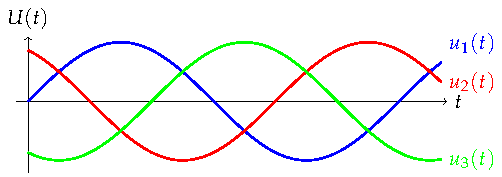
\includegraphics[]{../figs/TensionesTrifasica.pdf}\label{fig.tensionesTrifasica}} \hfill
		\subfloat[Fasores]{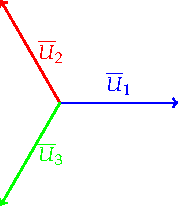
\includegraphics[]{../figs/FasoresTrifasica.pdf}\label{fig.fasoresTrifasica}}
		\caption{Forma de onda y fasores de una tensión trifásica}
		\label{fig.tensiontrifasica}
	\end{figure}
    \begin{figure}
		\centering
		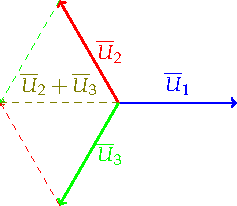
\includegraphics{../figs/FasoresSumaCero.pdf}
		\caption{Suma de fasores de una tensión trifásica}
		\label{fig.fasoressumacero}
	\end{figure}

    \newpage

    \vspace*{3mm}
    Nótese que la suma de las tensiones de fase es 0, como muestra la Figura~\ref{fig.fasoressumacero}:
	\begin{equation*}
		u_1(t) + u_2(t) + u_3(t) = 0 \quad\rightarrow\quad \overline{U}_1 + \overline{U}_2 + \overline{U}_3 = 0
	\end{equation*}
	
	\begin{remark}
	    Aunque en este caso concreto se ha demostrado para tensiones, en general, \textbf{la suma de tres fasores equilibrados es 0}.
	\end{remark}
	
	\subsection{Tensión de fase (simple) y de línea (compuesta)}\label{sec.fase_linea}
	Es necesario conocer también la diferencia entre las tensiones de \textbf{fase} (o tensiones simples) y de \textbf{línea} (o compuestas):
	\begin{itemize}
		\item \textbf{Tensión de fase.} Es la tensión en cada una de las fases (fase--neutro) del generador o en cada una de las impedancias del receptor. Suele representarse como: 
		\begin{equation*}
			\overline{U}_A\equiv \overline{U}_{f_1} \qquad \qquad \overline{U}_B\equiv \overline{U}_{f_2} \qquad \qquad \overline{U}_C \equiv \overline{U}_{f_3} 
		\end{equation*}
		\item \textbf{Tensión de línea.} Es la tensión existente entre los conductores de la línea, es decir, entre dos conductores de fase. Suele representarse como: 
		\begin{equation*}
			\overline{U}_{AB} \qquad \qquad \overline{U}_{BC} \qquad \qquad \overline{U}_{CA} 
		\end{equation*}
	\end{itemize}
	La relación entre las tensiones de fase y de línea son: 
	\begin{align}\label{eq.tensionFL}
		\overline{U}_{AB} &= \overline{U}_A - \overline{U}_B\\
		\overline{U}_{BC} &= \overline{U}_B - \overline{U}_C\\
		\overline{U}_{CA} &= \overline{U}_C - \overline{U}_A
	\end{align}
	cumpliéndose que la suma de tensiones de línea también es igual a 0. 
	\begin{remark}
	    Cuando, en un sistema trifásico, se habla únicamente de ``tensión'', \textbf{siempre} se refiere a la \textbf{tensión de línea}, independientemente de la forma de conexión de los generadores.
	\end{remark}
	
	Además de las tensiones de fase y línea, es necesario distinguir las corrientes de fase y línea:
	\begin{itemize}
		\item \textbf{Intensidad de fase.} Es la intensidad cedida por cada una de las fases del generador o que circula por cada impedancia del receptor. 
		\item \textbf{Intensidad de línea.} Es la intensidad que pasa por el conductor de la línea. 
	\end{itemize}
	
	\subsection{Secuencia de fases}\label{sec.secuencia_fases}
	
	El orden en el que se suceden las tensiones de cada fase de un circuito trifásico es lo que se conoce como \textit{secuencia de fases} (hace referencia a un punto concreto de la onda, por ejemplo, cuando todas ellas alcanzan el valor máximo). Existen dos tipos de secuencia de fases: $(i)$~secuencia de fases directa (\textbf{SFD}) y $(ii)$~secuencia de fases inversa (\textbf{SFI}), como se muestra en la Figura~\ref{fig.secuencia_fases}. 
	\begin{figure}[H]
		\centering
		\subfloat[SFD]{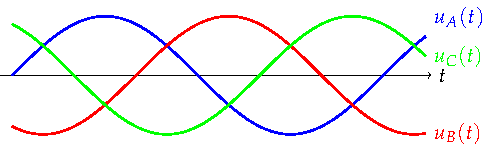
\includegraphics[width=0.45\linewidth]{../figs/TensionesTrifasica_ABC.pdf}}\hfil
		\subfloat[SFI]{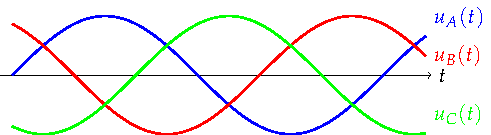
\includegraphics[width=0.45\linewidth]{../figs/TensionesTrifasica_ACB.pdf}}
		\caption{Secuencia de fases}
		\label{fig.secuencia_fases}
	\end{figure}
	
	%En la Figura~\ref{fig.secuencia_fases} se han representado los fasores asociados a las funciones sinusoidales de tensión, en una posición fija correspondiente a un instante determinado, que generalmente coincide con $t=0$. Sin embargo, debe tenerse en cuenta que, en realidad, son vectores rotatorios que giran con velocidad angular constante $\omega$ a izquierdas, es decir, en sentido antihorario. El orden en que los fasores que representan las tensiones pasan sucesivamente por un eje que pase por el origen (por ejemplo, el eje real) determina la secuencia de fases. 
	
	Conocer la secuencia de fases es \textbf{fundamental}, ya que según sea ésta, un mismo sistema de tensiones puede originar efectos distintos. Por ejemplo, un motor trifásico gira en un sentido al aplicarle
	una secuencia y en el contrario si se le aplica la otra. Además, para pasar de una secuencia a otra solo hay que intercambiar dos fases entre sí.
	
	\subsubsection{Secuencia de Fases Directa (SFD)}
	
	Se dice que se tiene \textit{secuencia directa} ($ABC$ o positiva), cuando la tensión $B$ está retrasada 120$^\circ$ respecto a la $A$, y la $C$ se retrasa 240$^\circ$ respecto a la $A$ (es decir, se adelanta 120$^\circ$). El \textbf{convenio} que se utiliza en esta asignatura para las tensiones en una \textbf{SFD} es:
	\begin{align*}
		u_A(t)&=U_f\,\sqrt{2}\cdot \sin(\omega\, t +\pi/2) \quad\rightarrow\quad \overline{U}_A=U_f\phase {90^\circ}\\
		u_B(t)&=U_f\,\sqrt{2}\cdot \sin(\omega\, t -\pi/6) \quad\rightarrow\quad \overline{U}_B=U_f\phase {-30^\circ}\\
		u_C(t)&=U_f\,\sqrt{2}\cdot \sin(\omega\,t +7\pi/6) \quad\rightarrow\quad \overline{U}_C=U_f\phase {210^\circ}
	\end{align*}
	
	Para conocer directamente la relación entre tensiones de fase y de línea, considérese las tensiones de fase $\overline{U}_A$ y $\overline{U}_B$: 
	\begin{align*}
		\overline{U}_A &= U_f\phase{90^\circ}=0+\mathrm{j}\,U_f
		\\
		\overline{U}_B &= U_f\phase{-30^\circ}=\dfrac{\sqrt{3}\,U_f}{2}-\mathrm{j}\,\dfrac{U_f}{2}
	\end{align*}
	Entonces, a partir de la expresión~\eqref{eq.tensionFL}, se obtiene que:
	\begin{equation*}
		\overline{U}_{AB} \;=\; \overline{U}_{A}-\overline{U}_{B} \;=\; (0+\mathrm{j}\,U_f)-\left(\dfrac{\sqrt{3}\,U_f}{2}-\mathrm{j}\,\dfrac{U_f}{2}\right)=-\dfrac{\sqrt{3}\cdot U_f}{2}+\mathrm{j}\,\dfrac{3\,U_f}{2} \;=\; \sqrt{3}\,U_f \phase{ 120^\circ}\,
	\end{equation*}
	es decir, que el módulo es $\sqrt{3}$ veces mayor que $U_f$ y está 30$^\circ$ adelantado respecto a la de fase. Por tanto:  
	\begin{equation}\label{eq.sfd_fase-linea}
		\boxed{
			\begin{array}{l}
				U_L = \sqrt{3}\cdot U_f\\
				\theta_L = \theta_f + 30^\circ\\
			\end{array}
		} 
	\end{equation}
	
	En la Figura~\ref{fig.linea-fase-SFD} se muestra el diagrama fasorial de las tensiones de fase y de línea. 
	\begin{figure}[H]
		\centering
		\subfloat[Obtención de la tensión de línea]{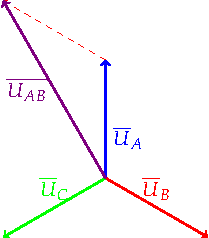
\includegraphics[height=3.25cm]{../figs/tension_LF.pdf}}\hfil
		\subfloat[Fasores de fase y línea]{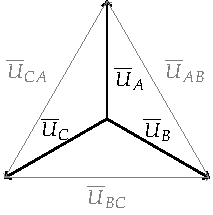
\includegraphics[height=3.25cm]{../figs/FasoresTrifasica_ABC.pdf}}
		\caption{Fasores de tensión de fase y línea en SFD}
		\label{fig.linea-fase-SFD}
	\end{figure}
	
	\subsubsection{Secuencia de Fases Inversa (SFI)}
	
	En la \textit{secuencia inversa} ($ACB$, negativa), la fase $C$ se retrasa 120$^\circ$ respecto a la $A$, y la $B$, se adelanta 120$^\circ$. La secuencia inversa se consigue permutando dos fases, generalmente $B$ por $C$. El \textbf{convenio} que se utiliza en esta asignatura para las tensiones en una \textbf{SFI}:
	\begin{align*}
		u_{A}(t)&=U_f\cdot\sqrt{2}\cdot \sin(\omega\cdot t -\pi/2) \quad\rightarrow\quad \overline{U}_{A}=U_f\phase {-90^\circ}\\
		u_{C}(t)&=U_f\cdot\sqrt{2}\cdot \sin(\omega\cdot t +5\pi/2) \quad\rightarrow\quad \overline{U}_{C}=U_f\phase {150^\circ}\\
		u_{B}(t)&=U_f\cdot\sqrt{2}\cdot \sin(\omega\cdot t +\pi/6) \quad\rightarrow\quad \overline{U}_{B}=U_f\phase {30^\circ}
	\end{align*}
	
	Para conocer directamente la relación entre tensiones de fase y de línea, considérese las tensiones de fase $\overline{U}_A$ y $\overline{U}_B$: 
	\begin{align*}
		\overline{U}_A &= U_f\phase{-90^\circ}=0-\mathrm{j}\,U_f
		\\
		\overline{U}_B &= U_f\phase{30^\circ}=\dfrac{\sqrt{3}\,U_f}{2}+\mathrm{j}\,\dfrac{U_f}{2}
	\end{align*}
	Entonces, a partir de la expresión~\eqref{eq.tensionFL}, se obtiene que: 
	\begin{equation*}
		\overline{U}_{AB} \;=\; \overline{U}_{A}-\overline{U}_{B} \;=\; (0-\mathrm{j}\,U_f)-\left(\dfrac{\sqrt{3}\,U_f}{2}+\mathrm{j}\,\dfrac{U_f}{2}\right) \;=\; -\dfrac{\sqrt{3}\cdot U_f}{2}-\mathrm{j}\,\dfrac{3\,U_f}{2} \;=\; \sqrt{3}\,U_f \phase{-120^\circ}\,
	\end{equation*}
	es decir, habiendo una relación entre tensiones de línea y de fase de: 
	\begin{equation}\label{eq.sfi_fase-linea}
		\boxed{
			\begin{array}{l}
				U_L = \sqrt{3}\cdot U_f\\
				\theta_L = \theta_f - 30^\circ\\
			\end{array}
		} 
	\end{equation}
	
	En la Figura~\ref{fig.linea-fase-SFI} se muestra el diagrama fasorial de las tensiones de fase y de línea. 

	\begin{figure}[H]
		\centering
		\subfloat[Obtención de la tensión de línea]{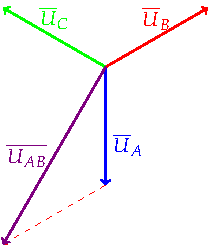
\includegraphics[height=3.25cm]{../figs/tension_LF_SFI.pdf}}\hfil
		\subfloat[Fasores de fase y línea]{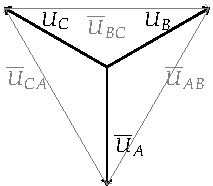
\includegraphics[height=3.25cm]{../figs/FasoresTrifasica_ACB.pdf}}
		\caption{Fasores de tensión de fase y línea en SFI}
		\label{fig.linea-fase-SFI}
	\end{figure}
	
	%Un generador se dice que está funcionando en \textbf{régimen equilibrado} si las tres intensidades de fase forman un sistema equilibrado de intensidades, de la misma secuencia que las tensiones del generador
	
	\section{Receptores trifásicos}\label{sec.conexiones}
	Los receptores de un sistema trifásico se pueden hacer en estrella (designada por la letra $Y$) y en triángulo (designada por la letra $D$). Se dice que el receptor está \textbf{equilibrado} cuando las tres impedancias son iguales en módulo \textbf{y} argumento, y \textbf{desequilibrado} cuando no lo son. Además, por conveniencia se considera que \textbf{las corrientes salen del generador} y recorren las tres fases y el neutro, y \textbf{entran al receptor}.
	
	\begin{remark}
	    Desde el punto de vista de los receptores, no importa demasiado el tipo de conexión de los generadores, sino las \textbf{tensiones disponibles} que, como se dijo en la Sección~\ref{sec.fase_linea}, se corresponde con la de \textbf{línea}.
	\end{remark}
	
	
	\subsection{Conexión en estrella}
	La conexión en estrella se consigue uniendo los terminales de polaridad de referencia ``negativa'' ($A'$, $B'$, $C'$), en un punto común llamado \textbf{neutro} ($N$), y quedan libres los otros tres terminales ($A$, $B$, $C$). También puede usarse como terminal de salida el punto neutro y utilizar un cuarto conductor, denominado \textbf{hilo neutro} (o, simplemente, \textbf{neutro}). Si este conductor existe, se dice que el sistema trifásico es un \textbf{sistema a cuatro hilos} y, si no existe, se dice que es un \textbf{sistema a tres hilos}. 
	
	\subsubsection{Estrella equilibrada}
	La Figura~\ref{fig.conexion_estrella_4} muestra la conexión de un receptor a cuatro hilos. Para este caso, se observa que se pueden medir directamente las \textbf{tensiones de fase} (entre cada fase y el neutro) y las \textbf{tensiones de línea} (entre cada dos fases) tanto del generador como del receptor. Suponiendo un receptor equilibrado, donde cada fase tiene una impedancia de $\overline{Z}=Z\phase{\theta^\circ}$, las intensidades son:
	\begin{align*}
      \overline{I}_A &= \dfrac{\overline{U}_A}{\overline{Z}} = \dfrac{U_f}{Z}\phase{\pm 90^\circ - \theta} \\
      \overline{I}_B &= \frac{\overline{U}_B}{\overline{Z}} = \frac{U_f}{Z}\phase{{\mp 30^\circ} - \theta}\\
      \overline{I}_C &= \frac{\overline{U}_C}{\overline{Z}} = \frac{U_f}{Z}\phase{{\mp 150^\circ} - \theta}
    \end{align*}
    con el signo de la fase superior para SFD e inferior para SFI. Por tanto, el módulo de las corrientes es igual para las tres fases: 
    \begin{equation}
        \boxed{I_A = I_B = I_C = \dfrac{U_f}{Z}}
    \end{equation}
    y sus argumentos se diferencian en $\pm120^\circ$, por lo que constituyen un \textbf{sistema equilibrado} de fasores, cuya suma es 0. Además, por la 1LK, se cumple que, en el nudo $N$: 
    \begin{equation}
        \cancelto{0}{\overline{I}_A  + \overline{I}_B + \overline{I}_C} + \overline{I}_N = 0 \quad\rightarrow\quad \boxed{\overline{I}_N = 0}
    \end{equation}
    de donde se concluye que, en este caso, la existencia del neutro es \textbf{innecesaria} al no circular corriente por él. 
	\begin{figure}[H]
		\centering
		{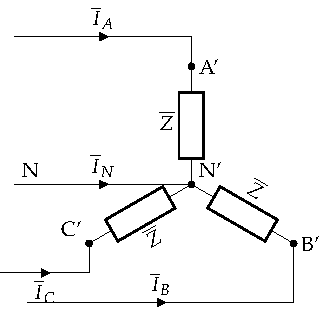
\includegraphics{../figs/EstrellaEquilibrado_Receptor.pdf}}
		\caption{Conexión en estrella a cuatro hilos}
		\label{fig.conexion_estrella_4}
	\end{figure}
	
	
	
	La Figura~\ref{fig.conexion_estrella_3} muestra la conexión de un generador y un receptor a tres hilos. Para este caso, se observa que únicamente se pueden medir directamente las \textbf{tensiones de línea} (entre cada dos fases) tanto del generador como del receptor. A partir del análisis del caso a cuatro hilos, donde se ha concluido que el neutro no era necesario, el estudio para la estrella equilibrada a tres hilos es idéntico. Suponiendo un receptor equilibrado, donde cada fase tiene una impedancia de $\overline{Z}=Z\phase{\theta^\circ}$, las intensidades son:
	\begin{align*}
      \overline{I}_A &= \frac{\overline{U}_A}{\overline{Z}} = \frac{U_f}{Z}\phase{{\pm 90^\circ} - \theta} \\
      \overline{I}_B &= \frac{\overline{U}_B}{\overline{Z}} = \frac{U_f}{Z}\phase{{\mp 30^\circ} - \theta}\\
      \overline{I}_C &= \frac{\overline{U}_C}{\overline{Z}} = \frac{U_f}{Z}\phase{{\mp 150^\circ} - \theta}
    \end{align*}
    con el signo de la fase superior para SFD e inferior para SFI. Por tanto, el módulo de las corrientes es igual para las tres fases: 
    \begin{equation}
        \boxed{I_A = I_B = I_C = \dfrac{U_f}{Z}}
    \end{equation}
    y sus argumentos se diferencian en $\pm120^\circ$, por lo que constituyen un \textbf{sistema equilibrado} de fasores, cuya suma es 0, lo cual se verifica además por la 1LK en el nudo $N$: 
    \begin{equation*}
        \overline{I}_A  + \overline{I}_B + \overline{I}_C = 0
    \end{equation*}
	\begin{figure}[H]
		\centering
		{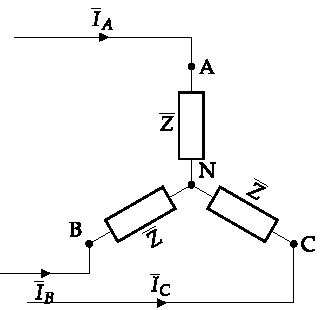
\includegraphics{../figs/EstrellaEquilibrado_Receptor_SN.pdf}}
		\caption{Conexión en estrella a tres hilos}
		\label{fig.conexion_estrella_3}
	\end{figure}

	Se observa que, en la conexión estrella, las intensidades que pasan por los conductores (corriente de línea) son \textbf{las mismas} que las cedidas por las fases del generador (corriente de fase), por lo que se cumple que:
	\begin{equation}
	    \boxed{\overline{I}_{L,i}=\overline{I}_{f,i}}
	\end{equation}
	

	
	
    \vspace{4mm}
    \begin{example}\label{ej.3-1}
	    Un sistema a cuatro hilos y SFI alimenta tres impedancias $\overline{Z}=10\phase{60^\circ}\,\Omega$, conectadas en estrella a una tensión de $200\sqrt{3}\,$ \si{\volt}. Determinar las corrientes de línea y el diagrama fasorial.
     
        \vspace{1mm}
	    \hspace*{-5mm}\hrulefill
        
        \vspace{4mm}
    
	    Siguiendo la referencia para SFI (Figura~\ref{fig.linea-fase-SFI}), las tensiones de fase y línea del sistema son:
	    \begin{align*}
	        \overline{U}_{AB} &= 200\,\sqrt{3}\phase{-120^\circ}\,\si{\volt} \quad\rightarrow\quad \overline{U}_A = 200\phase{-90^\circ}\,\si{\volt}\\
	        \overline{U}_{BC} &= 200\,\sqrt{3}\phase{0^\circ}\,\si{\volt} \quad\rightarrow\quad \overline{U}_B = 200\phase{30^\circ}\,\si{\volt}\\
	        \overline{U}_{CA} &= 200\,\sqrt{3}\phase{120^\circ}\,\si{\volt} \quad\rightarrow\quad \overline{U}_C=200\phase{150^\circ}\,\si{\volt}
	    \end{align*}
	    Por lo que las corrientes (de fase y de línea, al ser iguales):
	    \begin{align*}
	        \overline{I}_A &= \frac{200\phase{-90^\circ}}{10\phase{60^\circ}} =20\phase{-150^\circ} \,\si{\ampere} \\[10pt]
          \overline{I}_B &= \frac{200\phase{30^\circ}}{10\phase{60^\circ}} = 20\phase{-30^\circ} \,\si{\ampere}\\[10pt]
          \overline{I}_C &=\frac{200\phase{150^\circ}}{10\phase{60^\circ}} = 20\phase{90^\circ} \,\si{\ampere}
	    \end{align*}
	    siendo la corriente del neutro, por 1LK:
	    \begin{equation*}
	        \overline{I}_N=-(\overline{I}_A+\overline{I}_B+\overline{I}_C)=-(20\phase{-150^\circ}+20\phase{-30^\circ}+20\phase{90^\circ})=0
	    \end{equation*}
	    El diagrama fasorial se presenta en la Figura~\ref{fig.diagrama_ejemplo_3-1}. 
	    \begin{figure}[H]
	        \centering
	        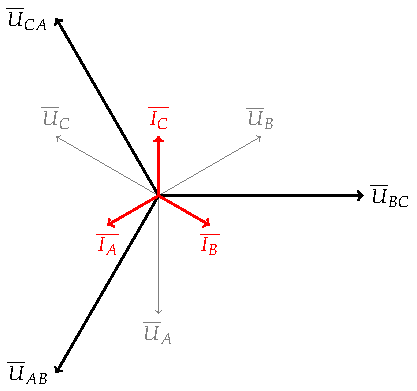
\includegraphics[width=0.4\linewidth]{../figs/diagrama_ejemplo3_1.pdf}
	        \caption{Diagrama fasorial del Ejemplo~\ref{ej.3-1}}
	        \label{fig.diagrama_ejemplo_3-1}
	    \end{figure}
	\end{example}
	
	\subsubsection{Estrella desequilibrada}
	
	La estrella está desequilibrada cuando las tres impedancias no sean iguales en módulo o argumento. Si se trata de un sistema a cuatro hilos, como el mostrado en la Figura~\ref{fig.estrelladeseqiulibrado_4hilos}, al ser las impedancias distintas, da lugar a intensidades de línea diferentes, no formando un sistema equilibrado de fasores. Las intensidades serán: 
	\begin{align*}
      \overline{I}_A &= \frac{\overline{U}_A}{\overline{Z}_A}\\
      \overline{I}_B &= \frac{\overline{U}_B}{\overline{Z}_B}\\
      \overline{I}_C &= \frac{\overline{U}_C}{\overline{Z}_C}
    \end{align*}
    y, aplicando la 1LK en $N$:
    \begin{equation}
        \overline{I}_A  + \overline{I}_B + \overline{I}_C + \overline{I}_N = 0
    \end{equation}
	pudiendo ser la corriente del neutro igual a 0 a pesar del desequilibrio de las impedancias. 
	
	\begin{figure}[H]
	    \centering
	    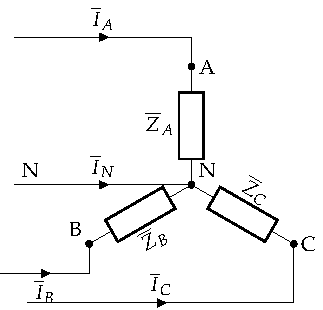
\includegraphics{../figs/EstrellaDesequilibrado_Receptor.pdf}
	    \caption{Receptor desequilibrado en estrella a cuatro hilos}
	    \label{fig.estrelladeseqiulibrado_4hilos}
	\end{figure}
	
	Si se tiene un sistema a tres hilos, no se puede seguir el procedimiento anterior, y se deberá aplicar el método de las mallas. 

        \vspace{4mm}
        \begin{example}\label{ej.estrella-deseq}
Un sistema trifásico de cuatro conductores, de secuencia de fases
directa y $\SI[parse-numbers=false]{200\sqrt{3}}{\volt}$ alimenta a
tres impedancias:
$\overline{Z}_{A} =
{10\phase{\ang{60}}}\unit{\ohm}$,
$\overline{Z}_{B} = {10\phase{\ang{0}}}\unit{\ohm}$
y
$\overline{Z}_{C} =
{10\phase{\ang{-30}}}\unit{\ohm}$. Determinar las
corrientes de línea.

\vspace{1mm}
\hspace*{-5mm}\hrulefill

\vspace{4mm}
        
Se trata de una conexión en estrella desequilibrada. Las tensiones de línea y fase son, respectivamente:
\[ U_L = \SI[parse-numbers=false]{200\sqrt{3}}{\volt} \quad \rightarrow \quad U_f =
  \SI{200}{\volt}
\]

Los fasores correspondientes, teniendo en cuenta que se trata de una secuencia de fases directa, son:
\begin{align*}
  \overline{U}_A &= {200\phase{\ang{90}}}\unit{\volt}\\
  \overline{U}_B &= {200\phase{\ang{-30}}}\unit{\volt}\\
  \overline{U}_C &= {200\phase{\ang{-150}}}\unit{\volt}\\
\end{align*}

Con estos fasores y las impedancias podemos calcular las corrientes de línea:
\begin{align*}
  \overline{I}_A &= \frac{\overline{U}_A}{\overline{Z}_A} = \frac{200}{10}\phase{\ang{90} - \ang{60}} \\
  \overline{I}_B &= \frac{\overline{U}_B}{\overline{Z}_B} = \frac{200}{10}\phase{\ang{-30} - \ang{0}}\\
  \overline{I}_C &= \frac{\overline{U}_C}{\overline{Z}_C} = \frac{200}{10}\phase{\ang{-150} - (\ang{-30})}
\end{align*}

 \begin{align*}
   \overline{I}_A &= {20\phase{\ang{30}}}\unit{\ampere}\\
   \overline{I}_B &= {20\phase{\ang{-30}}}\unit{\ampere}\\
   \overline{I}_C &= {20\phase{\ang{-120}}}\unit{\ampere}
 \end{align*}

 La corriente que circula por el neutro es:
 \[
   \overline{I}_N = -(\overline{I}_A + \overline{I}_B +
   \overline{I}_C) = {30.12\phase{\ang{144.89}}}\unit{\ampere}
 \]


\end{example}
	
	\subsection{Conexión en triángulo}\label{sec.triangulo}
	
	Una forma alternativa de conectar las tres fases de un generador/receptor es la \textbf{conexión en triángulo}, que se consigue conectando el terminal de polaridad de referencia negativa de una fase, con el de referencia positiva de otra fase ($A'$ con $B$, $B'$ con $C$ y $C'$ con $A$), como se muestra en la Figura \ref{fig.conexion_triangulo}. En este caso, se tiene únicamente un \textbf{sistema a tres hilos}, por lo que solo se dispone de la \textbf{tensión de línea}: 
	\begin{equation*}
	    \overline{U}_{AB};\qquad\qquad \overline{U}_{BC};\qquad\qquad \overline{U}_{CA}\qquad\qquad
	\end{equation*}
	\begin{figure}[H]
		\centering
		{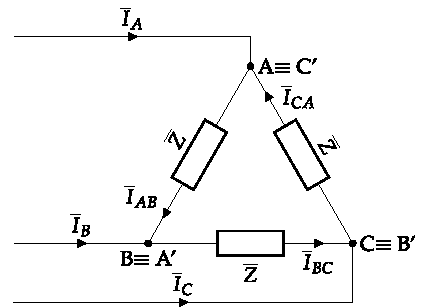
\includegraphics{../figs/TrianguloEquilibrado_Receptor.pdf}}
		\caption{Conexión en triángulo}
		\label{fig.conexion_triangulo}
	\end{figure}
	
	\subsubsection{Triángulo equilibrado}
	Las intensidades en cada impedancia (\textbf{intensidades de fase}) se obtienen como: 
	\begin{align*}
          \overline{I}_{AB} &= \frac{\overline{U}_{AB}}{\overline{Z}} = \frac{U}{Z}\phase{{\pm 120^\circ} - \theta} \\
          \overline{I}_{BC} &= \frac{\overline{U}_{BC}}{\overline{Z}} = \frac{U}{Z}\phase{0 - \theta}\\
          \overline{I}_{CA} &= \frac{\overline{U}_{CA}}{\overline{Z}} = \frac{U}{Z}\phase{{\mp 120^\circ} - \theta}
    \end{align*}
    con el signo de la fase superior para SFD e inferior para SFI. Estas corrientes tienen el mismo módulo: 
    \begin{equation}
        \boxed{{I_{AB}}={I_{BC}}={I_{CA}} = \dfrac{U_L}{Z}}
    \end{equation}
    Aplicando la 1LK en cada nudo del receptor, se obtienen las \textbf{corrientes de línea} que, al formar un sistema equilibrado: 
    \begin{align}
      \overline{I}_A &= \overline{I}_{AB} - \overline{I}_{CA} = \sqrt{3} \cdot \frac{U}{Z}\phase{{\pm 90^\circ} - \theta}\\
      \overline{I}_B &= \overline{I}_{BC} - \overline{I}_{AB} = \sqrt{3} \cdot \frac{U}{Z}\phase{{\mp 30^\circ} - \theta}\\
      \overline{I}_C &= \overline{I}_{CA} - \overline{I}_{BC} = \sqrt{3} \cdot \frac{U}{Z}\phase{{\mp 150^\circ} - \theta}
    \end{align}
    con el mismo criterio de signos que para las corrientes de fase. Por tanto, el módulo de las corrientes de línea es: 
    \begin{equation}
        \boxed{{I}_A = {I}_B = {I}_C = \sqrt{3} \cdot I_f = \sqrt{3}\,\frac{U_L}{Z}}
    \end{equation}
	
	\vspace{4mm}
    \begin{example}\label{ej.3-2}
	    Un sistema trifásico de secuencia directa y tensión $\qty{200}{\volt}$ alimenta tres impedancias iguales $\overline{Z}=10\phase{30^\circ}\,\Omega$, conectadas en triángulo. Determinar las corrientes de fase y línea, y dibujar el diagrama fasorial.

        \vspace{1mm}
	    \hspace*{-5mm}\hrulefill
        
        \vspace{4mm}
    
        Siguiendo la referencia para SFD (Figura~\ref{fig.linea-fase-SFD}), las tensiones de línea del sistema son:
	    \begin{align*}
	        \overline{U}_{AB}&=200\phase{120^\circ}\,\si{\volt}\\
	        \overline{U}_{BC}&=200\phase{0^\circ}\,\si{\volt}\\
	        \overline{U}_{CA}&=200\phase{-120^\circ}\,\si{\volt}
	    \end{align*}
	    Por lo que las corrientes de fase son:
	    \begin{align*}
	        \overline{I}_{AB} &= \frac{200\phase{120^\circ}}{10\phase{30^\circ}} =20\phase{90^\circ} \,\si{\ampere} \\[10pt]
          \overline{I}_{BC} &= \frac{200\phase{0^\circ}}{10\phase{30^\circ}} = 20\phase{-30^\circ} \,\si{\ampere}\\[10pt]
          \overline{I}_{CA} &=\frac{200\phase{-120^\circ}}{10\phase{30^\circ}} = 20\phase{-150^\circ} \,\si{\ampere}
	    \end{align*}
	    siendo las corrientes de línea, por 1LK:
	    \begin{align*}
	        \overline{I}_A&= \overline{I}_{AB}-\overline{I}_{CA} = \sqrt{3}\cdot 20\phase{60^\circ}\,\si{\ampere}\\
	        \overline{I}_B&= \overline{I}_{BC}-\overline{I}_{AB} = \sqrt{3}\cdot 20\phase{-60^\circ}\,\si{\ampere}\\
	        \overline{I}_C&= \overline{I}_{CA}-\overline{I}_{BC} = \sqrt{3}\cdot 20\phase{180^\circ}\,\si{\ampere}
	    \end{align*}
	    El diagrama fasorial se presenta en la Figura~\ref{fig.diagrama_ejemplo_3-2}. 
	    \begin{figure}[H]
	        \centering
	    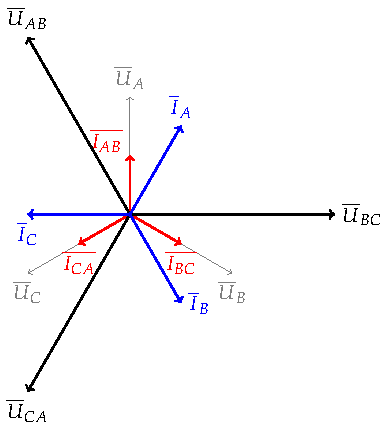
\includegraphics{../figs/diagrama_ejemplo3_2.pdf}
	        \caption{Diagrama fasorial del Ejemplo~\ref{ej.3-2}}
	        \label{fig.diagrama_ejemplo_3-2}
	    \end{figure}
	\end{example}
	
	\subsubsection{Triángulo desequilibrado}
	Se trata del receptor representado en la Figura~\ref{fig.trianguloDesequilibrado_receptor}. Supóngase que se conocen las tensiones de línea $\overline{U}_{AB}$, $\overline{U}_{BC}$ y $\overline{U}_{CA}$. En este caso, cada impedancia del triángulo es distinta de las demás, por lo que se tendrán tres corrientes de fase distintas en módulo y argumento:
	\begin{align*}
      \overline{I}_{AB} &= \frac{\overline{U}_{AB}}{\overline{Z}_{AB}}\\
      \overline{I}_{BC} &= \frac{\overline{U}_{BC}}{\overline{Z}_{BC}}\\
      \overline{I}_{CA} &= \frac{\overline{U}_{CA}}{\overline{Z}_{CA}}
    \end{align*}
    no constituyendo, por tanto, un sistema de fasores equilibrado. Las corrientes de línea se obtienen aplicando la 1LK en cada nudo:
    \begin{align}
      \overline{I}_A &= \overline{I}_{AB} - \overline{I}_{CA} \\
      \overline{I}_B &= \overline{I}_{BC} - \overline{I}_{AB}\\
      \overline{I}_C &= \overline{I}_{CA} - \overline{I}_{BC}
    \end{align}
    que, en general, no forman tampoco un sistema equilibrado de fasores.
	\begin{figure}[H]
	    \centering
	    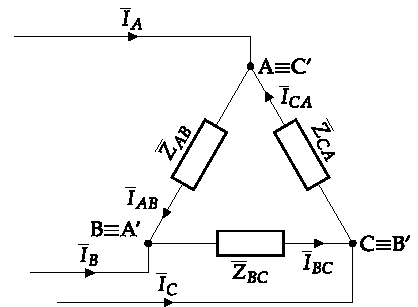
\includegraphics{../figs/trianguloDesequilibrado_receptor.pdf}
	    \caption{Receptor en triángulo desequilibrado}
	    \label{fig.trianguloDesequilibrado_receptor}
	\end{figure}
	
	\vspace{4mm}
	\begin{example}\label{ej.3-3}
	    Un sistema trifásico de SFI y tensión $\qty{200}{\volt}$ alimenta tres impedancias conectadas en triángulo, de valor $\overline{Z}_{AB}=10\phase{0^\circ}\,\Omega$, $\overline{Z}_{BC}=10\phase{30^\circ}\,\Omega$, $\overline{Z}_{AB}=10\phase{-45^\circ}\,\Omega$. Determinar las corrientes de fase y línea, y dibujar el diagrama fasorial.

        \vspace{1mm}
	    \hspace*{-5mm}\hrulefill
        
        \vspace{4mm}
	    
	    Siguiendo la referencia para SFI (Figura~\ref{fig.linea-fase-SFI}), las tensiones de línea del sistema son:
	    \begin{align*}
	        \overline{U}_{AB}&=200\phase{-120^\circ}\,\si{\volt}\\
	        \overline{U}_{BC}&=200\phase{0^\circ}\,\si{\volt}\\
	        \overline{U}_{CA}&=200\phase{120^\circ}\,\si{\volt}
	    \end{align*}
	    Por lo que las corrientes de fase:
	    \begin{align*}
	        \overline{I}_{AB} &= \frac{200\phase{-120^\circ}}{10\phase{0^\circ}} =20\phase{-120^\circ}\,\si{\ampere} \\[10pt]
          \overline{I}_{BC} &= \frac{200\phase{0^\circ}}{10\phase{30^\circ}} = 20\phase{-30^\circ}\,\si{\ampere}\\[10pt]
          \overline{I}_{CA} &=\frac{200\phase{120^\circ}}{10\phase{-45^\circ}} = 20\phase{165^\circ}\,\si{\ampere}
	    \end{align*}
	    siendo las corrientes de línea, por 1LK:
	    \begin{align*}
	     \overline{I}_A&=(20\phase{-120^\circ})-(20\phase{165^\circ})=24.350\phase{-67.50^\circ}\,\si{\ampere}\\	        \overline{I}_B&=(20\phase{-30^\circ})-(20\phase{-120^\circ})=28.284\phase{15^\circ}\,\si{\ampere}\\
	    \overline{I}_C&=(20\phase{165^\circ})-(20\phase{-30^\circ})=39.660\phase{157.5^\circ}\,\si{\ampere}
	    \end{align*}
	    El diagrama fasorial se presenta en la Figura~\ref{fig.diagrama_ejemplo_3-3}. 
	    \begin{figure}[H]
	        \centering
	        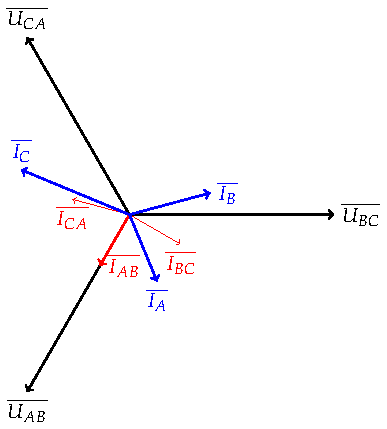
\includegraphics{../figs/diagrama_3_3.pdf}
	        \caption{Diagrama fasorial del Ejemplo~\ref{ej.3-3}}
	       \label{fig.diagrama_ejemplo_3-3}
	    \end{figure}
	\end{example}
	
	\section{Circuito equivalente monofásico de cargas trifásicas}\label{sec.c_eq_mon}
	 Siempre que se tenga un sistema equilibrado, es posible utilizar un \textbf{circuito monofásico equivalente} al trifásico, en el cual se representa una fase del original. Esto permite tomar cada fase en forma independiente de las restantes, sabiendo que las magnitudes de corriente y tensión calculadas serán iguales en amplitud y frecuencia, pero desfasada $120^\circ$ entre sí. Este método puede aplicarse tanto a estrella como a triángulo, teniendo siempre en cuenta que el circuito equivalente irá por \textbf{fase} y, por tanto, los elementos deberán tener una conexión en \textbf{estrella}. Nótese que, en este caso, las corrientes que se calcularán serán las de \textbf{línea}, que coincidirán con las de fase si la conexión inicial de la carga era en estrella, pero \textbf{no} si es en triángulo (ver Sección~\ref{sec.triangulo}); en este caso, las relaciones entre fase y línea mostradas en la Sección~\ref{sec.secuencia_fases} para la tensión son válidas también para la corriente.
	 
	  \begin{example}\label{ex.eq-mono}
	\textbf{	Un circuito trifásico de SFD presenta una línea de impedancia $1+\mathrm{j}2 \Omega$/hilo. A él se conectan dos cargas equilibradas con una tensión compuesta en sus terminales de 380V/50 Hz. La carga 1, en triángulo, presenta una impedancia $19\,\sqrt{3}\phase {60^\circ}\;\Omega$/fase; la carga 2, conectada en estrella, tiene una impedancia de $38/\sqrt{3}\phase{60^\circ}\;\Omega$/fase. Se pide:
			\begin{itemize}
				    \item Corrientes de fase en las cargas 1 y 2 y la corriente total absorbida
				    \item Tensión compuesta a principio de la línea
				\end{itemize}}
		
		La referencia de tensiones de línea, al ser secuencia directa:
		\begin{align*}
		  \overline{U_{A'B'}}&=380\phase{120^\circ} V\\
		  \overline{U_{B'C'}}&=380\phase{0^\circ} V\\
		  \overline{U_{C'A'}}&=380\phase{-120^\circ} V
		\end{align*}
		y las de fase:
		\begin{align*}	    \overline{U_A'}&=\dfrac{380}{\sqrt{3}}\phase{90^\circ}V\\    \overline{U_B'}&=\dfrac{380}{\sqrt{3}}\phase{-30^\circ}V\\   \overline{U_C'}&=\dfrac{380}{\sqrt{3}}\phase{-150^\circ}V
		\end{align*}
		
		Para determinar el equivalente monofásico, es necesario transformar la carga 1 en su estrella equivalente. Siguiendo la expresión~\eqref{eq.triangulo-estrella-igual}, extrapolado a una impedancia:
		\begin{equation*}
		    \overline{Z_{1,D}}=3\,\overline{Z_{1,Y}}\Rightarrow \overline{Z_{1,Y}}=\dfrac{\overline{Z_{1,D}}}{3}=\dfrac{19\,\sqrt{3}\phase{60^\circ}}{3}=\dfrac{19}{\sqrt{3}}\phase{60^\circ}\Omega
		\end{equation*}
		
		Así, queda un circuito monofásico (se calculará la fase $A$), formado por $\overline{Z_L}$ y las impedancias de $\overline{Z_{1,Y}}$ y $\overline{Z_2}$ en paralelo. Las corrientes de cada carga:
		\begin{align*}
		    \overline{I_{1,L,A}}&=\dfrac{\overline{U_A'}}{\overline{Z_{1,Y}}}=\dfrac{\frac{380}{\sqrt{3}}\phase{90^\circ}}{\frac{19}{\sqrt{3}}\phase{60^\circ}}=20\phase{30^\circ}\,A\\
		    \overline{I_{2,L,A}}&=\dfrac{\overline{U_A'}}{\overline{Z_{2}}}=\dfrac{\frac{380}{\sqrt{3}}\phase{90^\circ}}{\frac{38}{\sqrt{3}}\phase{60^\circ}}=10\phase{30^\circ}\,A
		\end{align*}
		y, por 1LK, la corriente total:
		\begin{equation*}
		    \overline{I_{L,A}}=\overline{I_{1,L,A}}+\overline{I_{2,L,A}}=20\phase{30^\circ}+10\phase{30^\circ}=30\phase{30^\circ} A
		\end{equation*}
		Volviendo al circuito original, las corrientes de la carga 1 de línea son:
		\begin{align*}
		    \overline{I_{1,L,A}}&=20\phase{30^\circ}\,A\\
		    \overline{I_{1,L,B}}&=20\phase{-90^\circ}\,A\\
		    \overline{I_{1,L,C}}&=20\phase{-210^\circ}\,A\\
		\end{align*}
		y, siguiendo las relaciones~\eqref{eq.sfd_fase-linea} al tratarse de una SFD, se obtiene que las corrientes de fase son: 
		\begin{align*}
		    \overline{I_{1,F,A}}&=\dfrac{20}{\sqrt{3}}\phase{0^\circ}\,A\\
		    \overline{I_{1,F,B}}&=\dfrac{20}{\sqrt{3}}\phase{-120^\circ}\,A\\
		    \overline{I_{1,F,C}}&=\dfrac{20}{\sqrt{3}}\phase{-240^\circ}\,A\\
		\end{align*}
		La corriente que circula por cada fase de la carga 2 es igual a la de línea al estar conectada en estrella. Por tanto:
		\begin{align*}
		    \overline{I_{2,F,A}}&=10\phase{30^\circ}\,A\\
		    \overline{I_{2,F,B}}&=10\phase{-90^\circ}\,A\\
		    \overline{I_{2,F,C}}&=10\phase{-210^\circ}\,A
		\end{align*}
		La corriente total absorbida en cada línea:
		\begin{align*}
		    \overline{I_{L,A}}&=30\phase{30^\circ} A\\
		    \overline{I_{L,B}}&=30\phase{-90^\circ} A\\
		    \overline{I_{L,C}}&=30\phase{-210^\circ} A\\
		\end{align*}
		
		
		La tensión de fase en el generador (principio de la línea) en el circuito equivalente monofásico:
		\begin{equation*}
		    \overline{U_{F,A}}=\overline{Z_L}\;\overline{I_{L,A}}+ \overline{U_A'}=(1+\mathrm{j}2)\cdot(30\phase{30^\circ})+\dfrac{380}{\sqrt{3}}\phase{90^\circ}=286.38\phase{90.8041^\circ} V
		\end{equation*}
		y, siguiendo las relaciones~\eqref{eq.sfd_fase-linea} al tratarse de una SFD, se obtiene que la tensión compuesta (de línea) es: 
		\begin{equation*}
		    \overline{U_{L,A}}=\sqrt{3}\,286.38\phase{120.8041^\circ} V 
		\end{equation*}
		siendo las tensiones en las líneas $B$ y $C$:
		\begin{align*}
			  \overline{U_{L,B}}&=\sqrt{3}\,286.38\phase{0.8041^\circ} V\\
			  \overline{U_{L,C}}&=\sqrt{3}\,286.38\phase{-119.1959^\circ} V
			\end{align*}
		\end{example}
	
	\section{Potencia en sistemas trifásicos}\label{sec.potencia_trifasica}
	Se analiza el caso de sistemas desequilibrados y equilibrados.
	
	\subsection{Sistemas desequilibrados}
	
	\subsubsection{Estrella}
	La forma de proceder es idéntica para sistemas a tres y a cuatro hilos. Supóngase un receptor desequilibrado en estrella, como el mostrado en la Figura~\ref{fig.estrellaDesequilibrado_potencia}, donde cada fase (impedancia, $\overline{Z_i}=Z_i\phase{\theta_i}$) consumirá una potencia activa dada por: 
	\begin{equation*}
	    P_A=U_{A}\cdot I_A \cdot \cos(\theta_A);\qquad \qquad
	    P_B=U_{B}\cdot I_B \cdot \cos(\theta_B);\qquad \qquad
	    P_C=U_{C}\cdot I_C \cdot \cos(\theta_C)
	\end{equation*}
	Por tanto, aplicando el Teorema de Boucherot (Sección~\ref{sec.boucherot}), la potencia total consumida por el receptor será:
	\begin{equation}
	    \boxed{P_T=P_A+P_B+P_C}
	\end{equation}
	De forma análoga, las potencias reactivas:
	\begin{equation*}
	    Q_A=U_{A}\cdot I_A \cdot \sin(\theta_A);\qquad \qquad
	    Q_B=U_{B}\cdot I_B \cdot \sin(\theta_B);\qquad \qquad
	    Q_C=U_{C}\cdot I_C \cdot \sin(\theta_C)
	\end{equation*}
	siendo la total: 
	\begin{equation}
	    \boxed{Q_T=Q_A+Q_B+Q_C}
	\end{equation}
	Por último, la potencia aparente: 
	\begin{equation*}
	    S_A=U_{A}\cdot I_A;\qquad \qquad
	    S_B=U_{B}\cdot I_B;\qquad \qquad
	    S_C=U_{C}\cdot I_C
	\end{equation*}
	siendo la total: 
	\begin{equation}
	    \boxed{S_T=\sqrt{P_T^2+Q_T^2}}\,\qquad\qquad \boxed{\overline{S_T}=P_T+\mathrm{j}\,Q_T}
	\end{equation}
	
	\begin{figure}[H]
	    \centering
	    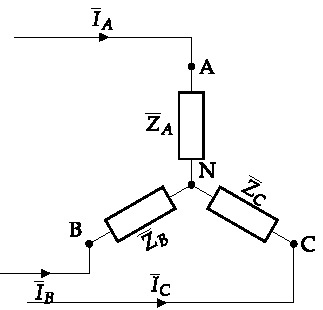
\includegraphics{../figs/EstrellaDesequilibrado_Receptor_SN.pdf}
	    \caption{Receptor en estrella desequilibrado}
	    \label{fig.estrellaDesequilibrado_potencia}
	\end{figure}
	
	\begin{remark}
	    Nótese, que al tratarse de un sistema desequilibrado, las \textbf{potencias totales} no pueden calcularse de otro modo
	\end{remark}
	
	\subsubsection{Triángulo}
	
	Supóngase un receptor desequilibrado en triángulo, como el mostrado en la Figura~\ref{fig.trianguloDesequilibrado_receptor_potencia}, donde cada fase (impedancia, $\overline{Z_i}=Z_i\phase{\theta_i}$) consumirá una potencia activa dada por: 
	\begin{equation*}
	    P_{AB}=U_{AB}\cdot I_{AB} \cdot \cos(\theta_{AB});\qquad \qquad
	    P_{BC}=U_{BC}\cdot I_{BC} \cdot \cos(\theta_{BC});\qquad \qquad
	    P_{CA}=U_{CA}\cdot I_{CA} \cdot \cos(\theta_{CA})
	\end{equation*}
	La potencia activa total, aplicando el Teorema de Boucherot es:
	\begin{equation}
	    \boxed{P_T=P_{AB}+P_{BC}+P_{CA}}
	\end{equation}
	De forma análoga, las potencias reactivas:
	\begin{equation*}
	    Q_{AB}=U_{AB}\cdot I_{AB} \cdot \sin(\theta_{AB});\qquad \qquad
	    Q_{BC}=U_{BC}\cdot I_{BC} \cdot \sin(\theta_{BC});\qquad \qquad
	    Q_{CA}=U_{CA}\cdot I_{CA} \cdot \sin(\theta_{CA})
	\end{equation*}
	siendo la total: 
	\begin{equation}
	    \boxed{Q_T=Q_{AB}+Q_{BC}+Q_{CA}}
	\end{equation}
	Por último, la potencia aparente: 
	\begin{equation*}
	    S_{AB}=U_{AB}\cdot I_{AB};\qquad \qquad
	    S_{BC}=U_{BC}\cdot I_{BC};\qquad \qquad
	    S_{CA}=U_{CA}\cdot I_{CA}
	\end{equation*}
	siendo la total: 
	\begin{equation}
	    \boxed{S_T=\sqrt{P_T^2+Q_T^2}}\,\qquad\qquad \boxed{\overline{S_T}=P_T+\mathrm{j}\,Q_T}
	\end{equation}
	
	\begin{figure}
	    \centering
	    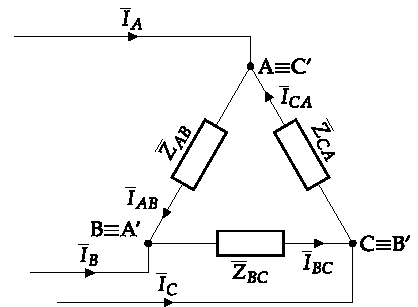
\includegraphics{../figs/trianguloDesequilibrado_receptor.pdf}
	    \caption{Receptor en triángulo desequilibrado}
	    \label{fig.trianguloDesequilibrado_receptor_potencia}
	\end{figure}
	
	\subsection{Sistemas equilibrados}
	
	\subsubsection{Estrella}
	
	La forma de proceder es idéntica para sistemas a tres y a cuatro hilos. Supóngase un receptor equilibrado en estrella, como el mostrado en la Figura~\ref{fig.estrellaequilibrado_SN_potencia}, donde cada fase (impedancia, $\overline{Z}=Z\phase{\theta}$) consumirá la misma potencia activa, dada por: 
	\begin{equation*}
	    P_F=U_{F}\cdot I_F \cdot \cos(\theta)
	\end{equation*}
	Dado que la potencia activa total consumida es la suma de la potencia consumida en cada fase, se obtiene que:
	\begin{equation*}
	    P_T=3\cdot P_F=3\cdot U_F\cdot I_F\cdot\cos(\theta)
	\end{equation*}
	Teniendo en cuenta que en la conexión estrella, se cumple que $U_L=\sqrt{3}\,U_F$ y que $I_L=I_F$, la potencia total consumida por el receptor es: 
	\begin{equation}
	    \boxed{P_T=3\cdot P_F=3\cdot U_F\cdot {I_F}\cdot\cos(\theta)=\sqrt{3}\cdot U_L\cdot I_L\cdot\cos(\theta)}
	\end{equation}
	
	
	De forma análoga, la potencia reactiva y aparente total:
	\begin{equation}
	    \boxed{Q_T=3\cdot Q_F=3\cdot U_F\cdot {I_F}\cdot\sin(\theta)=\sqrt{3}\cdot U_L\cdot I_L\cdot\sin(\theta)}
	\end{equation}
	\begin{equation}
	    \boxed{S_T=3\cdot S_F=3\cdot U_F\cdot {I_F}=\sqrt{3}\cdot U_L\cdot I_L}\qquad\qquad \boxed{\overline{S_T}=P_T+\mathrm{j}\,Q_T}
	\end{equation}
	
	\begin{figure}
	    \centering
	    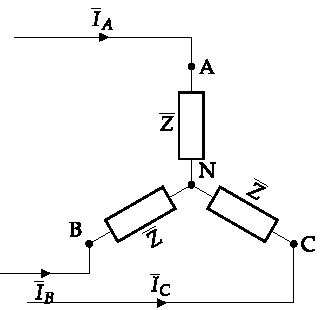
\includegraphics{../figs/EstrellaEquilibrado_Receptor_SN.pdf}
	    \caption{Receptor en estrella equilibrado}
	    \label{fig.estrellaequilibrado_SN_potencia}
	\end{figure}
	
	\subsubsection{Triángulo}
	
	Supóngase un receptor equilibrado en triángulo, como el mostrado en la Figura~\ref{fig.trianguloEquilibrado_receptor_potencia}, donde cada fase (impedancia, $\overline{Z}=Z\phase{\theta}$) consumirá la misma potencia activa, dada por: 
	\begin{equation*}
	    P_F=U_{F}\cdot I_F \cdot \cos(\theta)
	\end{equation*}
	Dado que la potencia activa total consumida es la suma de la potencia consumida en cada fase, se obtiene que:
	\begin{equation*}
	    P_T=3\cdot P_F=3\cdot U_F\cdot I_F\cdot\cos(\theta)
	\end{equation*}
	Teniendo en cuenta que en la conexión triángulo, se cumple que $U_L=U_F$ y que $I_L=\sqrt{3}\,I_F$, la potencia total consumida por el receptor es: 
	\begin{equation}
	    \boxed{P_T=3\cdot P_F=3\cdot U_F\cdot {I_F}\cdot\cos(\theta)=\sqrt{3}\cdot U_L\cdot I_L\cdot\cos(\theta)}
	\end{equation}
	que es idéntica a la expresión de la potencia activa consumida en la conexión estrella.
	
	De forma análoga, la potencia reactiva y aparente total:
	\begin{equation}
	    \boxed{Q_T=3\cdot Q_F=3\cdot U_F\cdot {I_F}\cdot\sin(\theta)=\sqrt{3}\cdot U_L\cdot I_L\cdot\sin(\theta)}
	\end{equation}
	\begin{equation}
	    \boxed{S_T=3\cdot S_F=3\cdot U_F\cdot {I_F}=\sqrt{3}\cdot U_L\cdot I_L}  \qquad\qquad \boxed{\overline{S_T}=P_T+\mathrm{j}\,Q_T}
	\end{equation}
	
	\begin{figure}
	    \centering
	    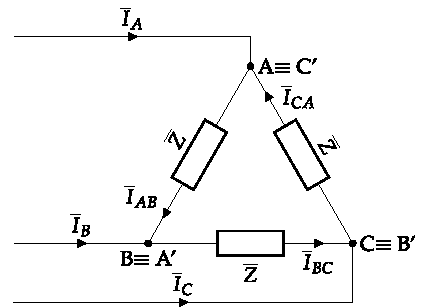
\includegraphics{../figs/TrianguloEquilibrado_Receptor.pdf}
	    \caption{Receptor en triángulo equilibrado}
	    \label{fig.trianguloEquilibrado_receptor_potencia}
	\end{figure}
	
	\begin{example}
	    \textbf{Una red trifásica de $20$ kV de tensión de línea alimenta a una instalación que dispone de dos cargas:
\begin{itemize}
    \item Carga 1: conexión triángulo, potencia nominal aparente de $300$ kVA y fdp $0.85$ inductivo
    \item Carga 2: conexión estrella, potencia nominal aparente de $100$ kVA y fdp $0.95$ capacitivo
\end{itemize}
Se pide calcular las potencias totales $P$, $Q$ y $S$, el módulo de la corriente de línea absorbida y el factor de potencia del conjunto.}

Las potencias de la carga 1:
\begin{align*}
    P_1&=S_1\,\cos(\phi_1)=300\cdot 0.85 = 255\,kW\\
    Q_1&=S_1\,\sin(\phi_1)=300\cdot\sin(\arccos(0.85))=158.03\,kVAr\\
    S_1&=300\,kVA
\end{align*}
y las de la carga 2:
\begin{align*}
    P_2&=S_2\,\cos(\phi_2)=100\cdot 0.95 = 95\,kW\\
    Q_2&=S_2\,\sin(\phi_2)=100\cdot\sin(\arccos(0.95))=-31.22\,kVAr\\
    S_2&=100\,kVA
\end{align*}
donde $Q_2$ es negativa al tratarse de un receptor capacitivo. Aplicando T. Boucherot, se tienen las potencias de la instalación:
\begin{align*}
    P_T&=P_1+P_2=255+95=350\,kW\\
    Q_T&=Q_1+Q_2=158.03+(-31.22)=126.81\,kVAr\\
    \overline{S_T}&=P_T+\mathrm{j}\,Q_T=350+\mathrm{j}\,126.81 \,kVA=372.26\phase{19.9162^\circ}\,kVA
\end{align*}
por lo que el factor de potencia del conjunto es:
\begin{equation*}
    fdp_T=\cos(\phi_T)=\cos(19.9162^\circ)=0.94
\end{equation*}
de carácter inductivo ($\phi_T>0$). 

Con las potencias se puede determinar el módulo de la corriente de línea:
\begin{equation*}
    I_L=\dfrac{S_T}{\sqrt{3}\,U_L}=\dfrac{372.26\cdot 10^3}{\sqrt{3}\cdot 20000}=10.75\,A
\end{equation*}
	\end{example}

	\subsection{Comparativa monofásica -- trifásica}
        En la introducción de este capítulo se mencionaban dos ventajas de los sistemas trifásicos respecto de los monofásicos:
	\begin{itemize}
		\item Los sistemas trifásicos proporcionan una potencia instantánea constante.
		\item Los sistemas trifásicos necesitan menos masa de conductor en igualdad de condiciones de potencia y tensión.
        \end{itemize}
        
        A continuación se demuestran ambas ventajas.

        \subsubsection{Potencia instantánea en un sistema trifásico}
        Supongamos un receptor equilibrado en estrella con SFD. Las tensiones de fase de este sistema serán:

\begin{equation*}
  u_A(t) = \sqrt{2} U_f \cos(\omega t + \ang{90});\qquad \qquad
  u_B(t) = \sqrt{2} U_f \cos(\omega t - \ang{30});\qquad \qquad
  u_C(t) = \sqrt{2} U_f \cos(\omega t - \ang{150})
\end{equation*}
Y las corrientes correspondientes:
\begin{equation*}
  i_A(t) = \sqrt{2} I \cos(\omega t + \ang{90} - \theta);\qquad \qquad
  i_B(t) = \sqrt{2} I \cos(\omega t - \ang{30} - \theta);\qquad \qquad
  i_C(t) = \sqrt{2} I \cos(\omega t - \ang{150} - \theta)
\end{equation*}

Además, la potencia de cada fase se expresa:
\begin{equation*}
  p_A(t) = u_A(t) \cdot i_A(t);\qquad \qquad
  p_B(t) = u_B(t) \cdot i_B(t);\qquad \qquad
  p_C(t) = u_C(t) \cdot i_C(t)
\end{equation*}

Sustituyendo las expresiones de tensiones y corrientes obtenemos:
\begin{align*}
  p(t) &=   p_A(t) + p_B(t) + p_C(t) = \\
&= \sqrt{2}U_f  \cos(\omega t + \ang{90}) \cdot \sqrt{2}I\cos(\omega t + \ang{90} - \theta) +\\
       &+ \sqrt{2}U_f \cos(\omega t - \ang{30}) \cdot \sqrt{2}I \cos(\omega t - \ang{30} - \theta) +\\
       &+ \sqrt{2}U_f \cos(\omega t - \ang{150}) \cdot \sqrt{2}I \cos(\omega t - \ang{150} - \theta)
\end{align*}

Para simplificar este resultado empleamos la expresión del producto de cosenos\footnote{$
  \cos(\alpha) \cdot \cos(\beta) = \frac{1}{2} \cdot (\cos(\alpha + \beta) + \cos(\alpha - \beta))$}:
\begin{align*}
  p(t) &= U_f I [\cos(2 \omega t + \ang{180} -\theta) + \cos(\theta)] +\\
       &+ U_f I [\cos(2 \omega t - \ang{60} - \theta) + \cos(\theta)] +\\
       &+ U_f I [\cos(2 \omega t - \ang{300} - \theta) + \cos(\theta)]
\end{align*}

La suma $\cos(2 \omega t + \ang{180} -\theta) + \cos(2 \omega t + \ang{60} -\theta) + \cos(2 \omega t + \ang{300} -\theta)$ es cero, por lo que el resultado final es:

\[
  p(t) = 3 \cdot U_f \cdot I \cdot \cos (\theta) = \sqrt{3} \cdot U \cdot I \cdot \cos (\theta) 
\]

Con esta expresión se demuestra que la potencia en el dominio del tiempo de un sistema trifásico equilibrado es constante, y su valor coincide con los resultados obtenidos anteriormente para la potencia activa. 


        \subsubsection{Masa necesaria de conductor}

        Compárese un sistema monofásico (subíndice $1$) y un sistema trifásico (subíndice $3$), que transmiten la \textbf{misma potencia activa} ($P_1=P_3$) y funcionan a la \textbf{misma tensión de fase} ($U_1=U_3=U$).
\[
U I_1 \cos(\theta) = P_1 = P_3 = \sqrt{3}U I_3 \cos(\theta) \rightarrow {I_1 = \sqrt{3} I_3}
\]
Las \textbf{pérdidas en la línea} deben ser \textbf{iguales} para recorrer la {misma distancia}:
\[
  2R_1I_1^2 = P_{1l} = P_{3l} = 3R_3I_3^2
\]
Sustituyendo la relación de corrientes y teniendo en cuenta la relación entre resistencia y sección ($R=\rho\frac{L}{S}$):
\[
  2\cdot R_1 \cdot 3I_3^2 = 3\cdot R_3 I_3^2 \rightarrow R_1 = \frac{1}{2} R_3 \rightarrow {S_1 = 2 \cdot S_3}
\]

Finalmente, la relación entre masas de conductor necesarias en cada sistema es:

\[
  \frac{m_3}{m_1} = \frac{3 \cdot S_3}{2 \cdot S_1} = \frac{3}{4}
\]

En consecuencia, un sistema trifásico equilibrado necesita un 25\% menos de masa de conductor para transportar la misma potencia que un sistema monofásico.

	\section{Medida de potencia en sistemas trifásicos} 
	
	Se estudian dos casos: sistema a cuatro y a tres hilos.
	
	\subsection{Sistemas a cuatro hilos}
	Para medir la potencia activa absorbida por cada fase de la carga, se necesitan tres vatímetros, indicando cada uno de ellos la potencia consumida por la fase donde está conectado, como se muestra en la Figura~\ref{fig.potencia4H}. Una vez medida la potencia en cada fase, la potencia total será:
	\begin{equation}
		\boxed{P_T=W_1+W_2+W_3}
	\end{equation}
	
	\begin{remark}
	    Si se tratase de una estrella equilibrada, los tres vatímetros darán la misma lectura ($W_1=W_2=W_3$), por lo que bastaría con colocar uno y hacer $P_T=3\cdot W_1$, como en la Figura~\ref{fig.potencia4Hequilibrado}.
	\end{remark}
	\begin{figure}[H]
		\centering
		\subfloat[Estrella desequilibrada]{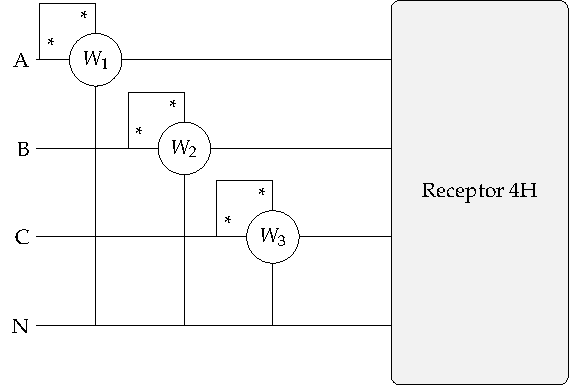
\includegraphics[height=5cm]{../figs/Potencia4H.pdf}\label{fig.potencia4H}}\hfill
		\subfloat[Estrella equilibrada]{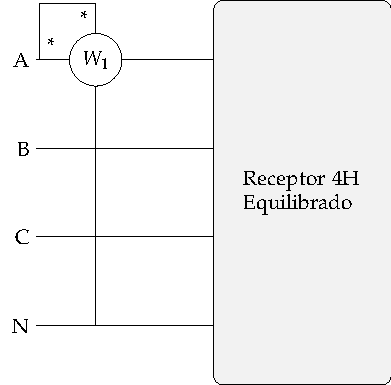
\includegraphics[height=5cm]{../figs/Potencia4H_Equilibrado.pdf}\label{fig.potencia4Hequilibrado}}
		\caption{Vatímetros para sistemas a cuatro hilos}
		\label{fig.vatimetro4hilos}
	\end{figure}
	
	\subsection{Sistemas a tres hilos}\label{sec.potencia_3H}
	
	\subsubsection{Estrella}
	
	La potencia total consumida viene dada por la parte real de la potencia compleja: 
	\begin{align*}
	    P_A=\Re\{\overline{U}_A \cdot \overline{I}_A^*\};\qquad \qquad
	    &P_B=\Re\{\overline{U}_B \cdot \overline{I}_B^*\};\qquad \qquad
	    P_C=\Re\{\overline{U}_C \cdot \overline{I}_C^*\}\\
	    &P_T=P_A+P_B+P_C
	\end{align*}
	Teniendo en cuenta que debe cumplirse la 1LK en el nudo $N$:
	\begin{equation*}
	    \overline{I_A}+\overline{I_B}+\overline{I_C}\Rightarrow \overline{I_C}=-(\overline{I_A}+\overline{I_B})
	\end{equation*}
	y, sustituyendo en la potencia total: 
	\begin{align}
          P_T &= \Re\{\overline{U_{A}} \cdot \overline{I_A}^*\} + \Re\{\overline{U_{B}} \cdot  \overline{I_B}^*\} + \Re\{\overline{U_{C}} \cdot \overline{I_C}^*\} = \nonumber\\
          &= \Re\{\overline{U_{A}} \cdot  \overline{I_A}^*\} + \Re\{\overline{U_{B}} \cdot  \overline{I_B}^*\} + \Re\{\overline{U_{C}} \cdot \left(-(\overline{I_A}^*+\overline{I_B}^*\}\right))=\nonumber \\
	    & =\Re\{(\overline{U_A}-\overline{U_C}) \cdot  \overline{I_A}^*\} + \Re\{(\overline{U_B}-\overline{U_C}) \cdot  \overline{I_B}^*\} \Rightarrow \nonumber\\  &\boxed{P_T = \Re\{\overline{U_{\textcolor{red}{A}C}} \cdot \overline{I_{\textcolor{red}{A}}}^*\} + \Re\{\overline{U_{\textcolor{cyan}{B}C}} \cdot \overline{I_{\textcolor{cyan}{B}}}^*\}}
	\end{align}
	es decir, que si se conectan dos vatímetros de manera que uno mida $W_1=\Re\{\overline{U_{AC}} \cdot \overline{I_A}^*\}$ y el otro $W_2=\Re\{\overline{U_{BC}} \cdot \overline{I_B}^*\}$, la suma de ambas lecturas es la potencia total: 
	\begin{equation*}
	    P_T=W_1+W_2
	\end{equation*}
	\begin{remark}
	    Se hace la observación de que $\overline{U_{AC}}=-\overline{U_{CA}}$. Además, si en lugar de $\overline{I_C}$ se hubiera despejado $\overline{I_A}$ o $\overline{I_B}$:
	    \begin{align*}
	        P_T&=\Re\{\overline{U_{\textcolor{cyan}{B}A}} \cdot \overline{I_{\textcolor{cyan}{B}}}^*\} + \Re\{\overline{U_{\textcolor{orange}{C}A}} \cdot \overline{I_{\textcolor{orange}{C}}}^*\}\\
	        P_T&=\Re\{\overline{U_{\textcolor{red}{A}B}} \cdot \overline{I_{\textcolor{red}{A}}}^*\} + \Re\{\overline{U_{\textcolor{orange}{C}B}} \cdot \overline{I_{\textcolor{orange}{C}}}^*\}
	    \end{align*}
	\end{remark}
	
	\subsubsection{Triángulo}
	
	La potencia total consumida viene dada por la parte real de la potencia compleja: 
	\begin{align*}
	    P_{AB}=\Re\{\overline{U}_{AB} \cdot \overline{I}_{AB}^*\};\qquad \qquad
	    &P_{BC}=\Re\{\overline{U}_{BC} \cdot \overline{I}_{BC}^*\};\qquad \qquad
	    P_{CA}=\Re\{\overline{U}_{CA} \cdot \overline{I}_{CA}^*\}\\
	    &P_T=P_{AB}+P_{BC}+P_{CA}
	\end{align*}
	Teniendo en cuenta que debe cumplirse la 1LK en los nudos $A$ y $B$:
	\begin{align*}
	    \overline{I_A}=\overline{I_{AB}}-\overline{I_{CA}}\Rightarrow \overline{I_{CA}}=\overline{I_{AB}}-\overline{I_A}\\
	    \overline{I_B}=\overline{I_{BC}}-\overline{I_{AB}}\Rightarrow \overline{I_{BC}}=\overline{I_{B}}+\overline{I_{AB}}
	\end{align*}
	y, sustituyendo en la potencia total:
		\begin{align}
	    P_T&= \Re\{\overline{U_{AB}}\cdot \overline{I_{AB}}^*\} + \Re\{\overline{U_{BC}}\cdot\left(\overline{I_B}^*+\overline{I_{AB}}^* \right)\}  + \Re\{\overline{U_{CA}} \cdot (\overline{I_{AB}}^*-\overline{I_A}^*)\}=\nonumber \\
                  &= \Re\{\cancelto{0}{(\overline{U_{AB}}+\overline{U_{BC}}+\overline{U_{CA}})}\cdot \overline{I_{AB}}^*\}+\Re\{\overline{U_{BC}} \cdot \overline{I_B}^*\} - \Re\{\overline{U_{CA}} \cdot \overline{I_A}^*\}\Rightarrow \nonumber \\
                  &\boxed{P_T=\Re\{\overline{U_{\textcolor{red}{A}C}} \cdot \overline{I_{\textcolor{red}{A}}}^*\} + \Re\{\overline{U_{\textcolor{cyan}{B}C}} \cdot \overline{I_{\textcolor{cyan}{B}}}^*\}}
	\end{align}
	idéntico resultado al que se obtiene para una estrella a tres hilos. Por tanto, si se conectan dos vatímetros de manera que uno mida $W_1=\Re\{\overline{U_{AC}} \cdot \overline{I_A}^*\}$ y el otro $W_2=\Re\{\overline{U_{BC}} \cdot \overline{I_B}^*\}$, la suma de ambas lecturas es la potencia total: 
	\begin{equation*}
	    P_T=W_1+W_2
	\end{equation*}
	
	\subsection{Método de los dos vatímetros}\label{sec.dos_vat}
	
	Al procedimiento mostrado en la Sección~\ref{sec.potencia_3H} se le denomina \textbf{método de los dos vatímetros} (o montaje de Aron), y se realiza del siguiente modo: 
	
	Se eligen \textbf{dos líneas cualesquiera} a las que se conectan las \textbf{bobinas de intensidad} del vatímetro. Las \textbf{entradas de las bobinas de tensión} se conectan a las \textbf{mismas líneas} que las de intensidad y, las \textbf{salidas}, a la \textbf{línea no usada}, como se muestra en la Figura~\ref{fig.potencia3H}. Como se mencionó en la Sección~\ref{sec.medida_potencia}, si alguno de los vatímetros da una lectura negativa, en la suma se considerará con el signo $-$.   
	\begin{figure}[H]
	    \centering
	    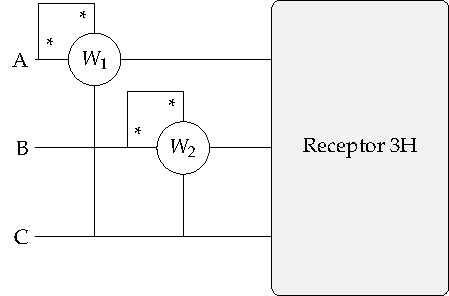
\includegraphics{../figs/Potencia3H.pdf}
	    \caption{Método de los dos vatímetros en líneas $A$ y $B$}
	    \label{fig.potencia3H}
	\end{figure}
	
	\subsubsection{Secuencia de fases directa}
	
	Supóngase una SFD y un receptor en estrella de carácter inductivo (el resultado es también aplicable a carácter capacitivo). El diagrama fasorial del circuito es el de la Figura~\ref{fig.fasores_potencia3H}. El ángulo de desfase entre la tensión de fase y la intensidad (de línea o fase, al ser la misma) es el correspondiente a la impedancia ($\theta$)
	\begin{figure}[H]
	    \centering
	    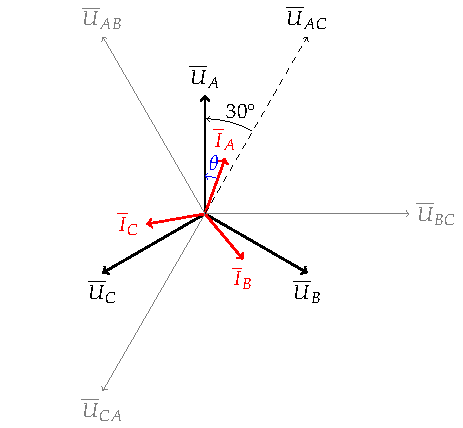
\includegraphics{../figs/fasores_potencia3H.pdf}
	    \caption{Diagrama fasorial de un receptor en estrella, inductivo y alimentado con SFD}
	    \label{fig.fasores_potencia3H}
	\end{figure}
	
	Colocando dos vatímetros en las líneas $A$ y $B$, como en la Figura~\ref{fig.Potencia3H_Equilibrado_AB}:
	\begin{equation*}
	    W_1=\Re\{\overline{U_{AC}} \cdot \overline{I_A}\}\qquad\qquad W_2=\Re\{\overline{U_{BC}} \cdot \overline{I_B}\}
	\end{equation*}
	donde se sabe que:
	\begin{align*} \overline{U_{AC}}&=-\overline{U_{CA}}=U_L\phase{-120^\circ-180^\circ}=U_L\phase{60^\circ}\\ \overline{U_{BC}}&=U_L\phase{0^\circ}\\ \overline{I_A}&=I_L\phase{90^\circ-\theta}\\ \overline{I_B}&=I_L\phase{-30^\circ-\theta} 
	\end{align*}
	Por tanto: 
	\begin{equation*}
	    W_1=U_L\;I_L\;\cos{(\theta-30^\circ)}\qquad W_2={U_L}\; {I_L}\;\cos{(\theta+30^\circ)}
	\end{equation*}
	
	Desarrollando los dos cosenos:
\begin{align*}
  \cos(\theta-{30^\circ}) &= \cos(\theta)\,\cos({30^\circ}) + \sin(\theta)\,\sin({30^\circ})\\
  \cos(\theta+{30^\circ}) &= \cos(\theta)\,\cos({30^\circ}) - \sin(\theta)\,\sin({30^\circ})
\end{align*}
y reemplazando en las expresiones de $W_1$ y $W_2$:
\begin{align*}
    W_1&=U_L\;I_L\;\cos{(\theta-30^\circ)}=U_L\;I_L\;\left( \cos(\theta)\,\cos({30^\circ}) + \sin(\theta)\,\sin({30^\circ})\right)\\
    W_2&=U_L\;I_L\;\cos{(\theta+30^\circ)}=U_L\;I_L\;\left( \cos(\theta)\,\cos({30^\circ}) - \sin(\theta)\,\sin({30^\circ})\right)
\end{align*}

Si se suman las medidas de los dos vatímetros, se obtiene que:
\begin{align}\label{eq.P_2vat_SFD}
    W_1+W_2&=\left[ U_L\,I_L\,\left( \cos(\theta)\,\cos({30^\circ}) + \cancel{\sin(\theta)\,\sin({30^\circ})}\right) \right] + [U_L\,I_L\,\left( \cos(\theta)\,\cos({30^\circ}) - \cancel{\sin(\theta)\,\sin({30^\circ})}\right) ]=\nonumber\\
    &=2\,U_L\,I_L\,\cos(\theta)\,\cos({30^\circ}) \Rightarrow \boxed{W_1 + W_2 = \sqrt{3}\,U_L\, I_L\,\cos(\theta) = P_T}
\end{align}
Además, si se restan: 
\begin{align}\label{eq.Q_2vat_SFD}
    W_1-W_2&=\left[U_L\,I_L\,\left( \cancel{\cos(\theta)\,\cos({30^\circ})} + \sin(\theta)\sin({30^\circ})\right)\right] - [U_L\,I_L\,\left( \cancel{\cos(\theta)\,\cos({30^\circ})} - \sin(\theta)\,\sin({30^\circ})\right) ]=\nonumber\\
    &=2\,U_L\,I_L\,\sin(\theta)\,\sin({30^\circ}) \Rightarrow \boxed{W_1 - W_2 = U_L\, I_L\,\sin(\theta) = \frac{Q_T}{\sqrt{3}}}
\end{align}
Por tanto, se puede calcular el ángulo del receptor a partir de las expresiones~\eqref{eq.P_2vat_SFD} y \eqref{eq.Q_2vat_SFD}, puesto que:
\begin{equation}
    \tan(\theta) = \dfrac{Q_T}{P_T}\Rightarrow \boxed{\tan(\theta) = \sqrt{3} \frac{W_1 - W_2}{W_1 + W_2}}
\end{equation}

Estos mismos resultados se obtendrían igualmente si se conectan los vatímetros en otras líneas. Si se conectan los vatímetros en $B$ y $C$ (Figura~\ref{fig.Potencia3H_Equilibrado_BC}) o entre $C$ y $A$ (Figura~\ref{fig.Potencia3H_Equilibrado_CA}), se segurá cumpliendo que: 
\begin{align*}
    W_1&=U_L\,I_L\,\cos(\theta-30^\circ) \\
    W_2&=U_L\,I_L\,\cos(\theta+30^\circ)
\end{align*}
siendo las potencias activas y reactivas totales: 
\begin{align*}
    P_T&=W_1 + W_2\\
    Q_T&=\sqrt{3}\,(W_1 - W_2)
\end{align*}
\begin{figure}[H]
    \centering\subfloat[Líneas $A$ y $B$]{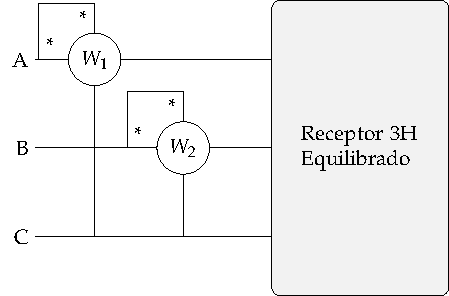
\includegraphics[width=0.3\linewidth]{../figs/Potencia3H_Equilibrado_AB.pdf}\label{fig.Potencia3H_Equilibrado_AB}}\hfill
    \subfloat[Líneas $B$ y $C$]{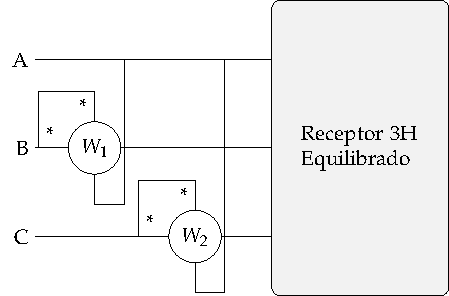
\includegraphics[width=0.3\linewidth]{../figs/Potencia3H_Equilibrado_BC.pdf}\label{fig.Potencia3H_Equilibrado_BC}}\hfill
    \subfloat[Líneas $C$ y $A$]{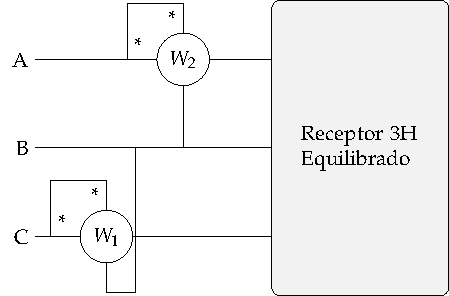
\includegraphics[width=0.3\linewidth]{../figs/Potencia3H_Equilibrado_CA.pdf}\label{fig.Potencia3H_Equilibrado_CA}}
    \caption{Método de los dos vatímetros en SFD}
    \label{fig.potencia3H_equilibrado_SFD}
\end{figure}

\begin{remark}
    Es posible recordar las conexiones de los vatímetros de la siguiente forma: al estar en una SFD, las fases presentan una sucesión $ABCABCABC$... En esta sucesión, se observa que {\color{red}\textbf{no}} se tiene $AC$, $BA$ ni $CB$, correspondientes a las conexiones de $W_1$ de la Figura~\ref{fig.potencia3H_equilibrado_SFD}, que miden el coseno de un ángulo $\theta-30^\circ$. Sin embargo, {\color{red}\textbf{sí}} se tiene $AB$, $BC$ y $CA$, correspondientes a las conexiones de $W_2$ de la Figura~\ref{fig.potencia3H_equilibrado_SFD}, que miden el coseno de un ángulo $\theta+30^\circ$.
\end{remark}
  
  \subsubsection{Secuencia de fases inversa}
	Considérese ahora una SFI y un receptor en estrella de carácter inductivo (el resultado es también aplicable a carácter capacitivo). El diagrama fasorial del circuito es el de la Figura~\ref{fig.fasores_potencia3H_SFI}. El ángulo de desfase entre la tensión de fase y la intensidad (de línea o fase, al ser la misma) es el correspondiente a la impedancia ($\theta$).
	\begin{figure}[H]
	    \centering
	    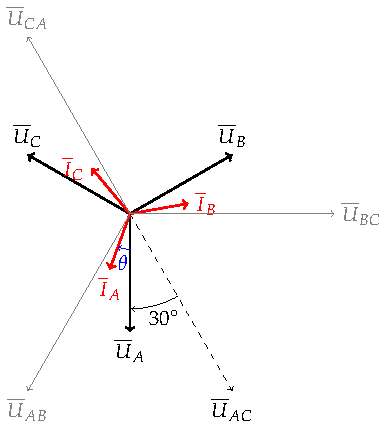
\includegraphics{../figs/fasores_potencia3H_SFI.pdf}
	    \caption{Diagrama fasorial de un receptor en estrella, inductivo y alimentado con SFI}
	    \label{fig.fasores_potencia3H_SFI}
	\end{figure}
	
	Colocando dos vatímetros en las líneas $A$ y $B$, como se muestra en la Figura~\ref{fig.Potencia3H_Equilibrado_AB_SFI}:
	\begin{equation*}
	    W_1=\Re\{\overline{U_{BC}} \cdot \overline{I_B}\}\qquad\qquad W_2=\Re\{\overline{U_{AC}} \cdot \overline{I_A}\}
	\end{equation*}
	donde se sabe que:
	\begin{align*}
	    \overline{U_{BC}}&=U_L\phase{0^\circ}\\
	   \overline{U_{AC}}&=-\overline{U_{CA}}=U_L\phase{120^\circ+180^\circ}=U_L\phase{-60^\circ}\\ \overline{I_B}&=I_L\phase{30^\circ-\theta} \\  \overline{I_A}&=I_L\phase{-90^\circ-\theta}
	\end{align*}
	Por tanto: 
	\begin{equation*}
	    W_1=U_L\;I_L\;\cos{(\theta-30^\circ)}\qquad W_2={U_L}\; {I_L}\;\cos{(\theta+30^\circ)}
	\end{equation*}
	cuyo resultado es idéntico al obtenido para la SFD: 
\begin{align}\label{eq.P_2vat_SFI}
    W_1+W_2&=\left[ U_L\,I_L\,\left( \cos(\theta)\,\cos({30^\circ}) + \cancel{\sin(\theta)\,\sin({30^\circ})}\right) \right] + [U_L\,I_L\,\left( \cos(\theta)\,\cos({30^\circ}) - \cancel{\sin(\theta)\,\sin({30^\circ})}\right) ]=\nonumber\\
    &=2\,U_L\,I_L\,\cos(\theta)\,\cos({30^\circ}) \Rightarrow \boxed{W_1 + W_2 = \sqrt{3}\,U_L\, I_L\,\cos(\theta) = P_T}
\end{align}
\begin{align}\label{eq.Q_2vat_SFI}
    W_1-W_2&=\left[U_L\,I_L\,\left( \cancel{\cos(\theta)\,\cos({30^\circ})} + \sin(\theta)\sin({30^\circ})\right)\right] - [U_L\,I_L\,\left( \cancel{\cos(\theta)\,\cos({30^\circ})} - \sin(\theta)\,\sin({30^\circ})\right) ]=\nonumber\\
    &=2\,U_L\,I_L\,\sin(\theta)\,\sin({30^\circ}) \Rightarrow \boxed{W_1 - W_2 = U_L\, I_L\,\sin(\theta) = \frac{Q_T}{\sqrt{3}}}
\end{align}
Por tanto, se puede calcular el ángulo del receptor a partir de las expresiones~\eqref{eq.P_2vat_SFI} y \eqref{eq.Q_2vat_SFI}, puesto que:
\begin{equation}
    \tan(\theta) = \dfrac{Q_T}{P_T}\Rightarrow \boxed{\tan(\theta) = \sqrt{3} \frac{W_1 - W_2}{W_1 + W_2}}
\end{equation}

\begin{figure}[H]
    \centering
    \centering\subfloat[Líneas $A$ y $B$]{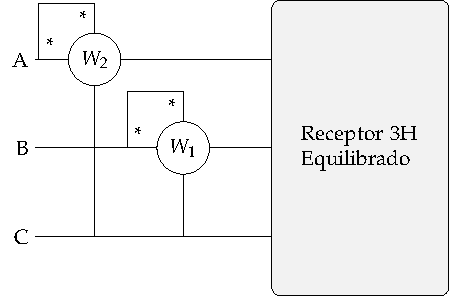
\includegraphics[width=0.3\linewidth]{../figs/Potencia3H_Equilibrado_AB_SFI.pdf}\label{fig.Potencia3H_Equilibrado_AB_SFI}}\hfill
    \subfloat[Líneas $B$ y $C$]{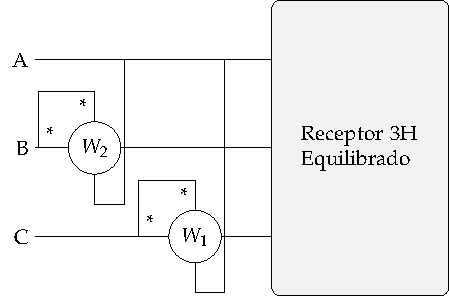
\includegraphics[width=0.3\linewidth]{../figs/Potencia3H_Equilibrado_BC_SFI.pdf}\label{fig.Potencia3H_Equilibrado_BC_SFI}}\hfill
    \subfloat[Líneas $C$ y $A$]{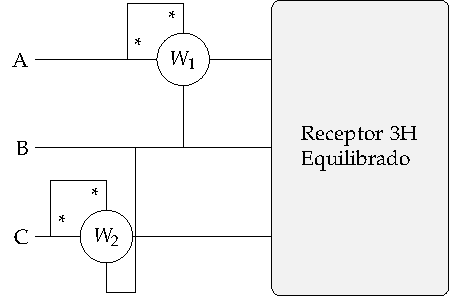
\includegraphics[width=0.3\linewidth]{../figs/Potencia3H_Equilibrado_CA_SFI.pdf}\label{fig.Potencia3H_Equilibrado_CA_SFI}}
    \caption{Método de los dos vatímetros en SFI}
    \label{fig.potencia3H_equilibrado_SFI}
\end{figure}

Estos mismos resultados se obtendrían igualmente si se conectan los vatímetros en otras líneas. Si se conectan los vatímetros en $B$ y $C$ (Figura~\ref{fig.Potencia3H_Equilibrado_BC}) o entre $C$ y $A$ (Figura~\ref{fig.Potencia3H_Equilibrado_CA}), se segurá cumpliendo que: 
\begin{align*}
    W_1&=U_L\,I_L\,\cos(\theta-30^\circ) \\
    W_2&=U_L\,I_L\,\cos(\theta+30^\circ)
\end{align*}
siendo las potencias activas y reactivas totales: 
\begin{align*}
    P_T&=W_1 + W_2\\
    Q_T&=\sqrt{3}\,(W_1 - W_2)
\end{align*}

\begin{remark}
    Es posible recordar las conexiones de los vatímetros de la siguiente forma: al estar en una SFI, las fases presentan una sucesión $ACBACBACB$.... En esta sucesión, se observa que {\color{red}\textbf{no}} se tiene $AB$, $BC$ ni $CA$, correspondientes a las conexiones de $W_1$ de las Figuras~\ref{fig.potencia3H} y \ref{fig.potencia3H_equilibrado_SFD}, que miden el coseno de un ángulo $\theta-30^\circ$. Sin embargo, {\color{red}\textbf{sí}} se tiene $AB$, $BC$ y $CA$, correspondientes a las conexiones de $W_2$ de las Figuras~\ref{fig.potencia3H} y \ref{fig.potencia3H_equilibrado_SFD}, que miden el coseno de un ángulo $\theta+30^\circ$.
\end{remark}

\begin{example}\label{ex.dos-vatimetros}
\textbf{Hallar la indicación del voltímetro en el sistema trifásico equilibrado de SFD de la Figura~\ref{fig.ej_dosvat}, sabiendo que: $W_1=700$ W; $W_2=400$ W; $\overline{Z_L}=1+\mathrm{j}2\Omega$; $\overline{Z_1}=100\Omega$; $\overline{Z_2}=47\phase{37^\circ}\Omega$.}
\begin{figure}[H]
    \centering
    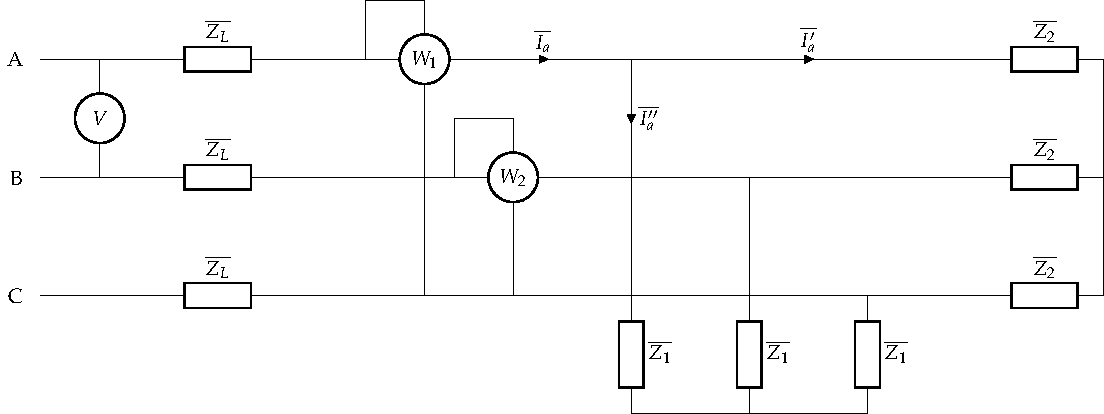
\includegraphics[width=.9\linewidth]{../figs/ej_dosvat.pdf}
    \caption{Ejemplo~\ref{ex.dos-vatimetros}}
    \label{fig.ej_dosvat}
\end{figure}

Al ser SFD, las potencias activa y reactiva totales:
\begin{align*}
    P_T&=W_1+W_2=700+400=1100\,W\\
    Q_T&=\sqrt{3}(W_1-W_2)=\sqrt{3}(700-400)=519.62\,VAr
\end{align*}

Con estos valores, se empieza a trabajar mediante un equivalente monofásico (de la fase $A$) del circuito trifásico original (ver Sección~\ref{sec.c_eq_mon}). Las cargas $\overline{Z_1}$ y $\overline{Z_2}$ están en paralelo, pudiéndose calcular la impedancia equivalente por fase:
\begin{equation*}
    \overline{Z_{eq,F}}=\dfrac{\overline{Z_1}\cdot\overline{Z_2}}{\overline{Z_1}+\overline{Z_2}}=\dfrac{100\cdot 47\phase{37^\circ}}{100+ 47\phase{37^\circ}}=33.47\phase{25.3787^\circ}\Omega=30.24+\mathrm{j}\,14.35\Omega
\end{equation*}
Al tratarse de un sistema equilibrado, la potencia activa y reactiva de cada fase es $1/3$ de la total. Con eso, y por su definición, puede determinarse el módulo de la corriente que circula por cada fase:
\begin{align*}
    P_F&=R_F\cdot I_F^2\Rightarrow I_F=\sqrt{\dfrac{P_F}{R_F}}=\sqrt{\dfrac{1100/3}{30.24}}=3.48\,A\\
    Q_F&=X_F\cdot I_F^2\Rightarrow I_F=\sqrt{\dfrac{Q_F}{X_F}}=\sqrt{\dfrac{519.62/3}{14.35}}=3.48\,A
\end{align*}
\begin{remark}
    Bastaría con calcular $I_F$ con la $P$ o la $Q$, aunque de esta forma se comprueba que el circuito hasta ahora está bien resuelto. 
\end{remark}
Esta $I_F$ es la que recorre a $\overline{Z_L}$ y a $\overline{Z_{eq}}$. Suponiendo que la corriente es el origen de fases $\overline{I_F}=3.48\phase{0^\circ}$ A, la tensión de fase del generador:
\begin{equation*}
    \overline{U_F}=\overline{I_F}\cdot (\overline{Z_L}+\overline{Z_{eq,F}})=3.48\phase{0^\circ}\cdot(1+\mathrm{j}2+30.24+\mathrm{j}\,14.35)=122.70\phase{27.6261^\circ} V
\end{equation*}

Dado que el voltímetro mide la \textbf{tensión entre fases} (es decir, la tensión de línea), marcará:
\begin{equation*}
    V=\sqrt{3}\,U_F=\sqrt{3}\cdot 122.70=212.52\,V
\end{equation*}
\end{example}


\subsection{Medida de potencia reactiva con un vatímetro}

Supóngase una SFD y un receptor en estrella de carácter inductivo, con el diagrama fasorial de la Figura~\ref{fig.fasores_potencia3H}. Si se hace el producto $\Re\{\overline{U_{BC}} \cdot \overline{I_A}^*\}$, se obtiene que:
\begin{equation*}
    \Re\{\overline{U_{BC}} \cdot \overline{I_A}^*\} = U_{BC}\;I_A\;\cos(\theta-90^\circ)=U_{BC}\;I_A\;\sin(\theta)
\end{equation*}
Por tanto, si se coloca un vatímetro que mida dicho producto escalar (como se muestra en la Figura~\ref{fig.Reactiva3H_A-BC}), se obtiene que: 
\begin{equation}
    W=\Re\{\overline{U_{BC}} \cdot \overline{I_A}^*\}=U_{L}\;I_L\;\sin(\theta)=\dfrac{Q_T}{\sqrt{3}}\Rightarrow \boxed{Q_T=\sqrt{3}\,W}
\end{equation}
donde $W$ representa la lectura del vatímetro. 
\begin{figure}[H]
    \centering
    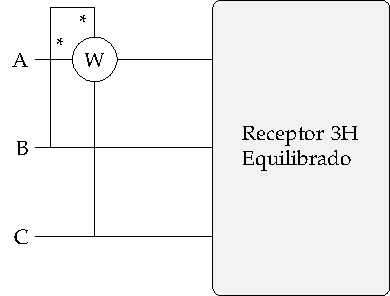
\includegraphics[height=3.7cm]{../figs/Reactiva3H_A-BC.pdf}
    \caption{Medida de reactiva con un vatímetro}
    \label{fig.Reactiva3H_A-BC}
\end{figure}

A modo de resumen, se muestran a continuación las diferentes conexiones que se pueden utilizar para medir la potencia reactiva, indicando su expresión tanto para SFD como SFI. Si se hace la conexión de las Figuras~\ref{fig.conexiones_reactiva1}--\ref{fig.conexiones_reactiva3}, la potencia reactiva es:
\begin{align}
SFD &\rightarrow \boxed{W = \frac{Q_T}{\sqrt{3}}}\\
SFI &\rightarrow \boxed{W =  - \frac{Q_T}{\sqrt{3}}}
\end{align}
Si se hace la conexión de las Figuras~\ref{fig.conexiones_reactiva4}--\ref{fig.conexiones_reactiva6}, la potencia reactiva es:
\begin{align}
SFD &\rightarrow \boxed{W = - \frac{Q_T}{\sqrt{3}}}\\
SFI &\rightarrow \boxed{W = \frac{Q_T}{\sqrt{3}}}
\end{align}

\begin{figure}[H]
    \centering
    \subfloat[]{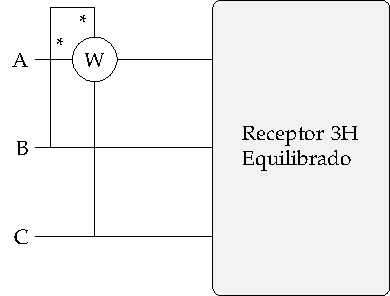
\includegraphics[width=0.3\linewidth]{../figs/Reactiva3H_A-BC.pdf}\label{fig.conexiones_reactiva1}}\hfill
    \subfloat[]{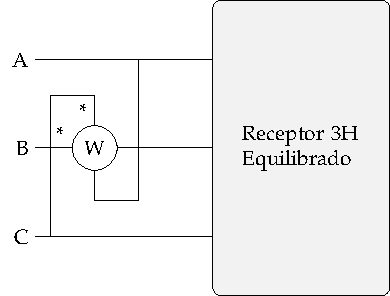
\includegraphics[width=0.3\linewidth]{../figs/Reactiva3H_B-CA.pdf}\label{fig.conexiones_reactiva2}}\hfill
    \subfloat[]{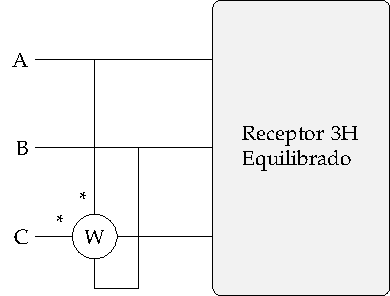
\includegraphics[width=0.3\linewidth]{../figs/Reactiva3H_C-AB.pdf}\label{fig.conexiones_reactiva3}}\hfill
    \subfloat[]{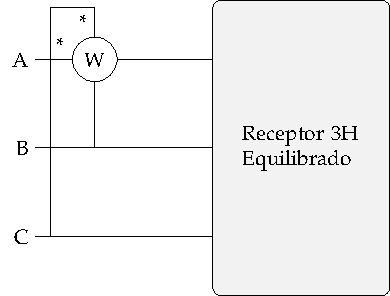
\includegraphics[width=0.3\linewidth]{../figs/Reactiva3H_A-CB.pdf}\label{fig.conexiones_reactiva4}}\hfill
    \subfloat[]{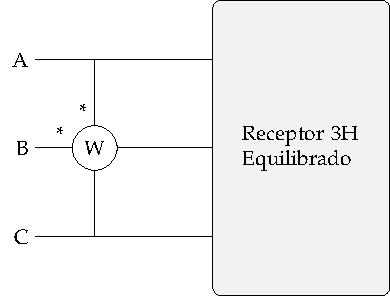
\includegraphics[width=0.3\linewidth]{../figs/Reactiva3H_B-AC.pdf}\label{fig.conexiones_reactiva5}}\hfill
    \subfloat[]{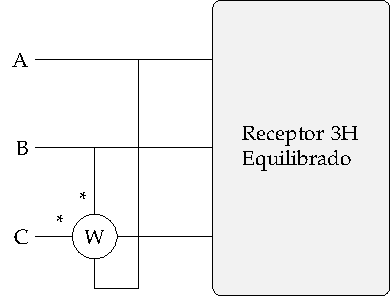
\includegraphics[width=0.3\linewidth]{../figs/Reactiva3H_C-BA.pdf}\label{fig.conexiones_reactiva6}}
    \caption{Conexiones para medida de reactiva}
\end{figure}

\begin{remark}
    Siguiendo las anotaciones realizadas para la medida de potencia activa y reactiva por el método de los dos vatímetros, las conexiones de las Figuras~\ref{fig.conexiones_reactiva1}--\ref{fig.conexiones_reactiva3} {\color{red}\textbf{sí}} se tienen en la SFD ($Q_T=\sqrt{3}\,W$) pero {\color{red}\textbf{no}} en la SFI ($Q_T=-\sqrt{3}\,W$). De manera similar, las conexiones de las Figuras~\ref{fig.conexiones_reactiva4}--\ref{fig.conexiones_reactiva6} {\color{red}\textbf{sí}} se tienen en la SFI ($Q_T=\sqrt{3}\,W$) pero {\color{red}\textbf{no}} en la SFD ($Q_T=-\sqrt{3}\,W$)
\end{remark}

		
		\begin{example}\label{ex.Q_vat}
\textbf{El sistema trifásico de la Figura~\ref{fig.Q_vat} es de 380 V, 50 Hz. Sabiendo que la carga es equilibrada y consume 24 kW
con un factor de potencia de 0,8 (inductivo), que las tensiones de línea son equilibradas y que se tiene una SFD, se pide calcular:
\begin{itemize}
    \item Valor de las intensidades de línea en forma fasorial
    \item Lectura de los vatímetros
    \item Si la línea de alimentación a la carga dispone de una impedancia $\overline{Z_L}=1+\mathrm{j}$ por conductor, determinar la tensión que debe disponer el generador en sus bornas para que la tensión en la carga sea de 380V
\end{itemize}}
\begin{figure}[H]
    \centering
    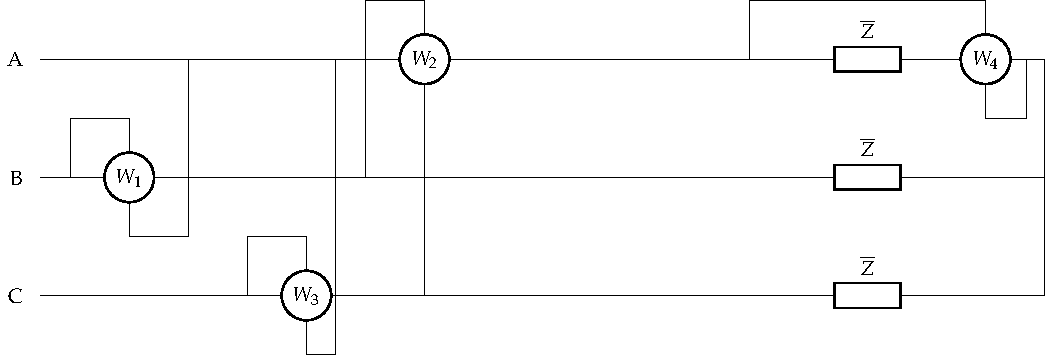
\includegraphics[width=\linewidth]{../figs/Q_vat.pdf}
    \caption{Ejemplo~\ref{ex.Q_vat}}
    \label{fig.Q_vat}
\end{figure}

Al tratarse de un sistema equilibrado en SFD:
\begin{align*}
    \overline{U_A}=\dfrac{380}{\sqrt{3}}\phase{90^\circ}\,V\qquad &\overline{U_{AB}}=380\phase{120^\circ}\,V\\
    \overline{U_B}=\dfrac{380}{\sqrt{3}}\phase{-30^\circ}\,V\qquad &\overline{U_{BC}}=380\phase{0^\circ}\,V\\
    \overline{U_C}=\dfrac{380}{\sqrt{3}}\phase{-150^\circ}\,V\qquad &\overline{U_{CA}}=380\phase{-120^\circ}\,V
\end{align*}

El módulo de la intensidad es:
\begin{equation*}
    P_T=\sqrt{3}\,U_L\,I_L\,\cos(\phi)\Rightarrow I=\dfrac{24000}{\sqrt{3}\cdot 380\cdot 0.8}=45.58\,A
\end{equation*}
Como el ángulo de la carga es $\arccos{(0.8)}=36.8699^\circ$ (por ser inductivo), y la fase de la corriente se puede determinar a partir de $\theta_I=\theta_U-\phi$:
\begin{align*}
    \overline{I_A}&=45.58\phase{53.1301^\circ}\,A\\
    \overline{I_B}&=45.58\phase{-66.8699^\circ}\,A\\
    \overline{I_C}&=45.58\phase{-186.8699^\circ}\,A
\end{align*}

La suma de los vatímetros $W_1$ y $W_3$ va a ser la potencia total de la carga (método de los dos vatímetros). El vatímetro $W_1$ mide la corriente $\overline{I_B}$ y la tensión $\overline{U_{BA}}$, por lo que: \begin{equation*}
    W_1=\overline{U_{BA}}\circ \overline{I_B}=U_{L}\cdot I_L\cdot \cos{(\theta_{U_{BA}}-\theta_{I_B})}= 380\cdot 45.58\cdot \cos(-60-(-66.8699))=17196.05\,W
\end{equation*}
El vatímetro $W_3$ mide la corriente $\overline{I_C}$ y la tensión $\overline{U_{CA}}$, por lo que: \begin{equation*}
    W_3=\Re\{\overline{U_{CA}}\cdot \overline{I_C}^*\}=U_{L}\cdot I_L\cdot \cos{(\theta_{U_{CA}}-\theta_{I_C})}= 380\cdot 45.58\cdot \cos(-120-(-186.8699))=6803.80\,W
\end{equation*}
cuya suma se comprueba que es igual a los 24 kW del enunciado.
\begin{remark}
    Los valores de $W_1$ y $W_3$ también podrían haberse obtenido directamente con lo indicado en la Sección~\ref{sec.dos_vat}:
    \begin{align*}
        W_1&=U_L\,I_L\,\cos(\phi-30)=380\cdot 45.58\cdot \cos(36.8699-30)=17196.05\,W\\
        W_3&=U_L\,I_L\,\cos(\phi+30)=380\cdot 45.58\cdot \cos(36.8699+30)=6803.80\,W
    \end{align*}
\end{remark}

El vatímetro $W_2$ mide en realidad la potencia reactiva, en este caso dividida por $\sqrt{3}$. Dado que la potencia reactiva total es:
\begin{equation*}
    Q_T=P_T\,\tan(\phi)=24000\cdot\tan(36.8699)=18000 \,\text{VAr}\Rightarrow W_2=\dfrac{Q_T}{\sqrt{3}}=10392.30\,W
\end{equation*}

El vatímetro $W_4$ mide la potencia de la fase $A$. Al tratarse de un sistema equilibrado:
\begin{equation*}
    W_4=\dfrac{P_T}{3}=\dfrac{24000}{3}=8000W
\end{equation*}

Las potencias en los bornes del generador son:
\begin{align*}
    P_T&=P_L+P_C=3\,R_L\,I_L^2+P_C=3\cdot 1\cdot 45.58^2+24000=30232.61\,W\\
    Q_T&=Q_L+Q_C=3\,X_L\,I_L^2+P_C=3\cdot 1\cdot 45.58^2+18000=24232.61\,VAr\\
    \overline{S_T}&=P_T+\mathrm{j}Q_T=30232.61+\mathrm{j}24232.61=38745.71\phase{38.7135^\circ} VA
\end{align*}
por lo que la tensión del generador:
\begin{equation*}
    S=\sqrt{3}\,U_L\, I_L\Rightarrow U_L=\dfrac{38745.71}{\sqrt{3}\,45.58}=490.78\,V
\end{equation*}
\end{example}

		\section{Mejora del factor de potencia}
		
		
		
		El objetivo y procedimiento es el mismo que en las instalaciones monofásicas (Sección~\ref{sec.mejora_fdp_monofasica}). Para reducir la potencia reactiva del sistema, se debe instalar un \textbf{banco de condensadores} que suministren una potencia reactiva $Q_C$. Como resultado, la potencia reactiva y el factor de potencia del sistema serán $Q' = Q - Q_C$ y $\cos(\theta') > \cos (\theta)$. La única diferencia con respecto a las instalaciones monofásicas es que en este caso se puede optar por un banco de condensadores acoplados en triángulo ($C_D$) o en estrella ($C_Y$):
		\begin{figure}[H]
		    \centering
		    \subfloat[Triángulo]{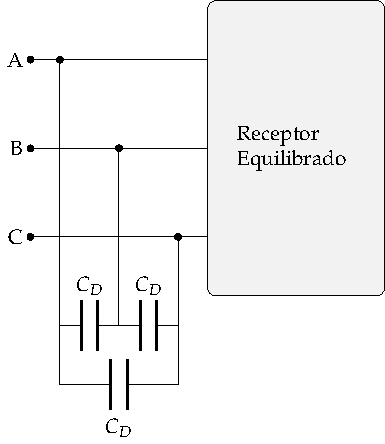
\includegraphics[width=0.35\linewidth]{../figs/CircuitoTrifasica_CompensacionReactiva.pdf}\label{fig.compensacion_reactiva_triangulo_trif}}\hfil
		    \subfloat[Estrella]{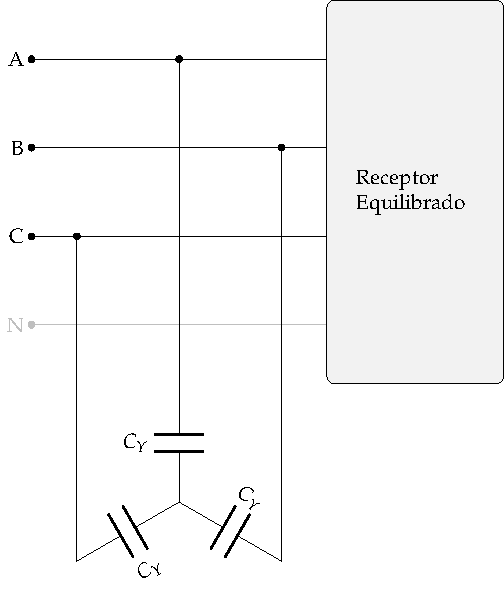
\includegraphics[width=0.42\linewidth]{../figs/CircuitoTrifasicaY_CompensacionReactiva.pdf}\label{fig.compensacionY_reactiva_triangulo_trif}}
		    \caption{Compensación de reactiva}
		\end{figure}
		\begin{itemize}
		    \item \textbf{Conexión en triángulo.} Si se conectan los condensadores en triángulo, como en la Figura~\ref{fig.compensacion_reactiva_triangulo_trif}, se tiene que: 
		\begin{align*}
          Q &= P\tan(\theta)\\
          Q' &= P\tan(\theta') = Q - Q_C\\
          Q_C &= 3 \cdot \omega\, C_D \cdot U_L^2
        \end{align*}
        \begin{equation}
            \boxed{C_D = \frac{P(\tan (\theta) - \tan (\theta'))}{3\,\omega\, U_L^2}}
        \end{equation}
		    \item \textbf{Conexión en estrella.} Cuando se conectan los condensadores en estrella, como en la Figura~\ref{fig.compensacionY_reactiva_triangulo_trif}, se tiene que: 
		\begin{align*}
          Q &= P\tan(\theta)\\
          Q' &= P\tan(\theta') = Q - Q_C\\
          Q_c &= 3 \cdot \omega C_Y \cdot U_F^2 = \cancel{3} \cdot \omega \,C_Y \cdot \left(\dfrac{U_L}{\cancel{\sqrt{3}}}\right)^2=\omega C_Y \cdot U_L^2
        \end{align*}
        \begin{equation}
            \boxed{C_Y = \frac{P(\tan (\theta) - \tan (\theta'))}{\omega\, U_L^2}}
        \end{equation}
		\end{itemize}
		
		
		
		Por tanto, y dado que $C_Y = 3 \cdot C_D$, la capacidad en triángulo es \textbf{tres veces menor} que en estrella. Así, la configuración recomendada en \textbf{triángulo}.
		
		\begin{example}\label{ex.compensacion_Q_trif}
		    \textbf{Una red trifásica de 380 V, 50 Hz y secuencia SFD alimenta a dos cargas equilibradas: $(i)$ 30 kW y factor de potencia $0.7$ inductivo; $(ii)$ 24 kW y factor de potencia $0.6$ inductivo. Determinar la capacidad de cada uno de los condensadores a conectar a la red para que el factor de potencia global mejore hasta $0.95$.}
		    
		    La potencia reactiva inicial es:
		    \begin{equation*}
		        Q_T=Q_1+Q_2=30\cdot \tan(\arccos(0.7))+24\cdot \tan(\arccos(0.6))=62.61\,\text{kVAr}
		    \end{equation*}
		    La potencia reactiva una vez se tenga la batería de condensadores será: 
		    \begin{equation*}
		        Q_T'=P_T\,\tan(\phi_T')=(30+24)\cdot \tan(\arccos(0.95))=17.75\,\text{kVAr}
		    \end{equation*}
		    siendo la potencia aportada por los condensadores:
		    \begin{equation*}
		        Q_C=Q_T'-Q_T=17.75-62.61=-44.86\,\text{kVAr}
		    \end{equation*}
		    por lo que la capacidad a conectar en cada fase del triángulo: 
		    \begin{equation*}
		     C_D=\dfrac{Q_C}{3\,\omega\,U_L^2}=\dfrac{44.80\cdot 10^3}{3\cdot 2\cdot \pi\cdot 50\cdot 380^2}=329.63\,\mu F/fase
		    \end{equation*}
		\end{example}

		 
	
	% %%%%%%%%%%%%%%%%%
	
% 	\chapterimage{tema4.jpg} % Chapter heading image
% 	\chapter{Teoremas generales de circuitos}
	
	
% \subsection{Teorema de multiplicación por una constante}
% Es consecuencia de la propiedad de proporcionalidad de los circuitos lineales. El teorema dice así: \textit{En un circuito compuesto por generadores (independientes y dependientes) e impedancias, si se multiplican todas las excitaciones (generadores independientes) por una constante $K$, las respuestas (corrientes de rama o tensiones de nudo), quedan multiplicadas por $K$} (Figura~\ref{fig.proporcionalidad}).

% \begin{figure}[H]
%         \centering
%         \subfloat[Respuesta inicial]{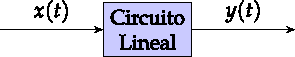
\includegraphics{../figs/proporcionalidad.pdf}}\hfil
%         \subfloat[Respuestsa proporcional]{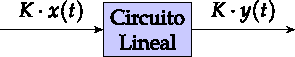
\includegraphics{../figs/proporcionalidad2.pdf}}
%         \caption{Proporcionalidad}
%         \label{fig.proporcionalidad}
%     \end{figure}
    
%   Con este teorema, aparecen dos posibles tipos de problemas a resolver:
%   \begin{itemize}
%       \item ¿Qué excitación se debe aplicar a un circuito para obtener una determinada respuesta?
%       \item ¿Qué respuesta proporciona un circuito ante una determinada excitación?
%   \end{itemize}
  
%   \subsubsection{¿Qué excitación se debe aplicar a un circuito para obtener una determinada respuesta?}
%   El procedimiento más sencillo para responder a esta pregunta es el siguiente: 
%   \begin{itemize}
% \item Aplicar una excitación de valor unidad.
% \item Resolver el circuito, obteniendo la respuesta del circuito a la excitación unidad.
% \item Hallar la constante de proporcionalidad $K$ entre la respuesta obtenida y la respuesta deseada.
% \item La excitación que se debe aplicar es esa constante de proporcionalidad (puede ser un número complejo).
% \end{itemize}
  
%   \subsubsection{¿Qué respuesta proporciona un circuito ante una determinada excitación?}
%   El proceso para obtener dicha respuesta es:
%   \begin{itemize}
% \item Suponer una respuesta de valor unidad.
% \item Resolver el circuito a la inversa, obteniendo la excitación que provoca la respuesta unidad.
% \item Hallar la constante de proporcionalidad $K$ entre la excitación obtenida y la excitación deseada.
% \item La respuesta que entrega el circuito es esa constante de proporcionalidad (puede ser un número complejo).
% \end{itemize}

% \section{Teorema de reciprocidad}

% \section{Teorema o regla de la sustitución}


%%% Local Variables:
%%% mode: latex
%%% TeX-master: "TC"
%%% ispell-local-dictionary: "castellano"
%%% End:
